%% uctest.tex 11/3/94
%% Copyright (C) 1988-2004 Daniel Gildea, BBF, Ethan Munson.
%
% This work may be distributed and/or modified under the
% conditions of the LaTeX Project Public License, either version 1.3
% of this license or (at your option) any later version.
% The latest version of this license is in
%   http://www.latex-project.org/lppl.txt
% and version 1.3 or later is part of all distributions of LaTeX
% version 2003/12/01 or later.
%
% This work has the LPPL maintenance status "maintained".
% 
% The Current Maintainer of this work is Daniel Gildea.
%
% 2007/08/01
% LaTeX Package "ucr" is modified from LaTeX package "ucthesis."
% This modification is therefore under to the conditions of 
% the LaTeX Project Public License.
% Its formality is suitable for the dissertation of Universty of
% California, Riverside.
% This test document is for the convenience of all students of
% Universty of California, Riverside.
% Contact Charles Yang at chcyang@yahoo.com if you like.
% Charles Yang has nothing to do with the original author's sarcasm.
%
% \documentclass[11pt]{ucthesis}
% \documentclass[11pt]{ucr}
\documentclass[oneside,final, letterpaper]{ucr}
%% Packages %%
% DO NOT INCLUDE tabularx or tabulary
\usepackage{booktabs}
\usepackage{lipsum}
\usepackage{calc}
\usepackage{braket}
\usepackage{float,graphicx}
\usepackage{subcaption}
\usepackage{amsmath}
\usepackage{amssymb}
\usepackage{array}
\usepackage[figuresright]{rotating}
\usepackage[usenames,dvipsnames,svgnames]{xcolor}

% Configure hyperlinks
\usepackage{hyperref}

% Widow and Orphan Penalty
\usepackage[all]{nowidow}

% Configuration For PDF
%\hypersetup{
%    colorlinks,
%    linkcolor={red!50!black},
%    citecolor={blue!50!black},
%    urlcolor={blue!80!black},
%    bookmarks=true,
%    pdfpagelabels=true
%    hyperfootnotes=false,
%    hyperindex=true,
%    pageanchor=false,
%    colorlinks,
%}

% Configuration for Printing
\hypersetup{
    colorlinks,
    linkcolor={black},
    citecolor={black},
    urlcolor={black},
    bookmarks=true,
    pdfpagelabels=true
    hyperfootnotes=false,
    hyperindex=true,
    pageanchor=false,
    colorlinks,
}

% Remove by adding ``final'' to argument list of 'document class' in thesis.tex
%\usepackage{draftwatermark}
%\SetWatermarkColor{red}
%\SetWatermarkAngle{0}
%\SetWatermarkHorCenter{0.1\paperwidth}
%\SetWatermarkVerCenter{0.05\paperheight}
%\SetWatermarkFontSize{5cm}
%\SetWatermarkText{\textbf{DRAFT}}

%% Define Custom Colors %%
\definecolor{ucrgold}{RGB}{241,161,0}
\setcounter{secnumdepth}{4}

%% Custom Commands %%

% Create an obvious citation placeholder
\newcommand{\needcite}[0]{\textbf{\textcolor{red}{ [CITATION NEEDED]}}}

% Create an obvious need caption placeholder
\newcommand{\needcap}[0]{\textbf{\textcolor{red}{[CAPTION NEEDED]}}}

% Create an obvious need figure placeholder
\newcommand{\needfig}[0]{\textbf{\textcolor{red}{[FIGURE NEEDED]}}}

% Create an editing Bookmark
\newcommand{\edithere}[0]{\textbf{\textcolor{red}{\chapter{Resume Here!}}}}

% Generate a sideways table placeholder
\newcommand{\sidewaystab}[0]
{
\begin{sidewaystable}
\centering
\begin{tabular}{ l l p{6cm} p{8cm} }
\toprule
\textbf{Source} & \textbf{Field} & \textbf{Description} & \textbf{Application} \\
\midrule 
ABBJKHSAD & QKLQAJDJ & JKSDEKJHA & lorem ipsonm kasjdk klekk iuiklkas, asjkhe  \\
 & INFO & asde iwjw qkjq kqj kk jqguh  & ialksj kwj jhhjkas pqmxc,mn ;la  \\
 & INFO & Standard PHENIX run ordering & \\
 & INFO & asde iwjw qkjq kqj kk jqguh  & ialksj kwj jhhjkas pqmxc,mn ;la  \\
 & INFO & asde iwjw qkjq kqj kk jqguh  & ialksj kwj jhhjkas pqmxc,mn ;la  \\
 & INFO & Standard PHENIX run ordering & \\
 & INFO & asde iwjw qkjq kqj kk jqguh  & ialksj kwj jhhjkas pqmxc,mn ;la  \\
\bottomrule
\end{tabular}
\caption{ \textbf{\textcolor{red}{NEED A REAL TABLE HERE}}}
\label{tab:sidewaystab}
\end{sidewaystable}

}

% Generate a regular table placeholder
\newcommand{\regtab}[0]
{
\begin{table}
\centering
\begin{tabular}{c c c c c c c c}
\toprule
{a} & {b} & {c} & {d} & {e} & {f} & {g} & {h} \\
(i) & (j) & (l) & (m) & (n) & (o) & (p) & (q) \\
\midrule
999.99 & 999.99 & - & 999.99 & 999.99 & (13 \%) & 999.99 & (13 \%)\\
999.99 & 999.99 & - & 999.99 & 999.99 & (18 \%) & 999.99 & (18 \%)\\
999.99 & 999.99 & - & 999.99 & 999.99 & (23 \%) & 999.99 & (23 \%)\\
999.99 & 999.99 & - & 999.99 & 999.99 & (31 \%) & 999.99 & (31 \%)\\
999.99 & 999.99 & - & 999.99 & 999.99 & (41 \%) & 999.99 & (41 \%)\\
999.99 & 999.99 & - & 999.99 & 999.99 & (76 \%) & 999.99 & (78 \%)\\
\bottomrule
\end{tabular}
\caption{ \textbf{\textcolor{red}PLACEHOLDER TABLE}}
\label{tab:regtab}
\end{table}

}

% Generate a squared figure placeholder
\newcommand{\sqfig}
{
\begin{figure}
\begin{center}

\includegraphics[width=\linewidth,height=\textheight,keepaspectratio]{figures/filler/squareimg.png}
\caption{ \textcolor{red}{Default Caption} }
\label{fig:sqfig}
\end{center}
\end{figure}

}
% Generate a portrait figure placeholder
\newcommand{\pofig}
{
\begin{figure}
\begin{center}

\includegraphics[width=\linewidth,height=\textheight,keepaspectratio]{figures/filler/portraitimg.png}
\caption{ \textcolor{red}{Default Caption} }
\label{fig:sqfig}
\end{center}
\end{figure}
}

% Generate a landscape figure placeholder
\newcommand{\lafig}
{
\begin{figure}
\begin{center}

\includegraphics[width=\linewidth,height=\textheight,keepaspectratio]{figures/filler/landscapeimg.png}
\caption{ \textcolor{red}{Default Caption} }
\label{fig:sqfig}
\end{center}
\end{figure}
}


\begin{document}

% Add additional packages, custom commands 

% Declarations for Front Matter
\title{MEASUREMENT OF THE LONGTIDUDIANL SINGLE SPIN ASYMMETRY, $A_L$, FOR POLARIZED PROTON-PROTON COLLISIONS IN THE $W\rightarrow\mu$ DECAY CHANNEL}
\author{Michael J. Beaumier}
\degreemonth{August}
\degreeyear{2016}
\degree{Doctor of Philosophy}
\chair{Professor Kenneth Barish }
\othermembers{Professor Rich Seto\\
Professor John Ellison}
\numberofmembers{3}
\field{Physics}
\campus{Riverside}

\maketitle
\copyrightpage{}
\approvalpage{}

\degreesemester{Summer}

\begin{frontmatter}

% Acknowlegements Page
\begin{acknowledgements}
	Advisors and Mentors are some of the most important people any scientist will
encounter in their professional career. Time and again, I have heard colleagues
speak of "that one inspirational" person that drove them to be their best, and
knew how to "grow" a researcher. 

I am very greatful to my advisor, Ken Barish, whose calm, stoic and unabated
support helped guide me through my research. Ken involved me in many aspects of
the research group at UCR, beyond the scientific work. He insured that I was
exposed to all aspects of research in particle physics, including writing
grants, reviewing literature, mentoring younger students, building detectors,
running a particle accelelrator detector, and of course, data analysis.  Ken has
always had the uncanny ability to know "who to talk to" for nearly any problem I
might have. Ken connected me with other excellent physicists, who helped me grow
as a researcher, and he gave me the freedom I needed to pursue my interests, and
move in the scientific directions I felt most fruitful, while helping to provide
an overall direction for my academic career and research. 

Beyond all this, the single most important thing Ken has done for me, is to give
me a second chance in graduate school. When he accepted me into his group, I was
an undoubtedly risky choice. I struggled mightily my first year in grad school.
I earned poor grades, and even had to re-take a class. In fact, my performance
was so poor, that my teaching responsibilities were reduced, and eventually, I
lost my graduate division fellowship, which ultimately meant that I had no
income, or means of supporting myself; I was effectively dismissed from graduate
school. However, I was interested in the research carried out by Ken and Rich
Seto's heavy ion group, so I talked to Ken, who graciously accepted me into the
group, provided me with academic and financial support, and even flew me out to
Brookhaven National Lab my first summer of graduate school. I finally got to
dive into 'real' physics research. I think it was this vote of confidence from
Ken, as well as the awesome physics happening at the PHENIX experiment which
gave me the confidence to wholeheartedly devote myself to my studies and
research. Without Ken's vote of confidence, I fear that my graduate career would
have been over in short order.

While at Brookhaven National Lab, I encountered graduate students, post docs,
research staff, and other amazing physicists who taught me an incredible
amount, and showed both patience, kindess, friendship and mentorship to me.
Richard Hollis was one of the first people I encoutered in my research group at
UCR - I have never met a more patient person. Richard helped me get my
bearings, and set me straight, during my early (and later) years of graduate
school. Oleg Eyser was with our group at that time as well - although I recall
that he was less than thrilled to have yet another green graduate student
constantly asking questions, taking time away from his work. He still made time
to teach me, and introduced me to the very complicated PHENIX software system.
Oleg challenged me, and expected me to find answers for myself, and was
unrelenting in that regard, which I am certain made me a better researcher.

Josh Perry gave me a crash course on the PHENIX data acquisition system,
boiling down this incredibly complicated system into understandable pieces, and
helped me learn that ultimately, persistance pays off when tackling difficult
problems. Martin Leitgab took me under his wing while I worked days and nights
to learn PHENIX's fast data production systems. Martin's systematic, calm, and
patient approach to problem solving has been something I have tried to emulate
since my work with him - I could not have asked for a better mentor for that
project. On that same project was my first introduction to Chris Pinkenburg and
Martin Purschke - somewhat of the yin and yang of the PHENIX online data
aquisition. I benefited enormously from conversations with both about PHENIX
software, and online systems. Martin Purschke's kindness and sense of humor
always spurred me on, while Chis' dogged dedication to doing things 'the right
way' kept me honest. I have returned to Martin with various questions many
times over the years, and he has always been cheerful, supportive and wise with
his answers. Probably nobody other than Ed Desmond has been woken up so many
times with emergencies at the PHENIX counting house in the middle of the night,
yet even when I woke him at 3 am on many occasions, would simply state, in an
execptionally dry, well practiced line: 'Martin Speaking, please state the
nature of your emergency'. I don't know of many who can manage to be coy and
good natured under such circumstances.

I have to acknoledge Joe Seele as well, in this regard, as he probably more
than anyone else, set me on the path to learning to program well, and using a
computer effectively - these skills, so often neglected in Particle Physics,
have paid off for me, many, many times over.

W Analysis Crew \\
  Ralf Seidl, 
  Francesca Giordano, 
  Sangwha Park, 
  Daniel Jumper, 
  Abraham Meles,
  Chong Kim, 

Friends and Family \\
  Bob Beaumier, 
  Marian Beaumier, 
  Joe Beaumier, 
  David Beaumier, 
  Emily Vance, 
  Jackie Hubbard, 
  Alexander Anderson-Natalie, 
  Corey Kownacki, 
  Chris Heidt, 
  Pat Odenthal, 
  Behnam Darvish Sarvestani, 
  Oleg Martynov, 

\end{acknowledgements}

% Dedication Page
\begin{dedication}
\null\vfil
{\large
\begin{center}
	Some say that it takes a village to raise a child. The same can be said of
	raising a graduate student up to earning a PhD. This thesis is dedicated to
	the multitude who have helped me become the man I am today, and to students
	who struggle, and their mentors who do not give up on them. \\
\end{center}}
\vfil\null
\end{dedication}

% Abstract Page
\begin{abstract}
	This thesis discusses the process of extracting information about the spin
	structure of protons, specifically, spin contributions from the sea of quarks
	and antiquarks, which are kinematically distinct from the 'valence quarks'.
	We have known since the 'proton-spin crisis' ~\cite{Ashman1988} of the 1990s
	that proton spin does not entirely reside in the valence quarks, so the
	thrust of experimental efforts since then have been designed to determine
	both how to probe the proton spin structure, and how to validate models for
	proton spin structure. Here, I discuss one particular approach to
	understanding the sea-quark spin contribution, which utilizes the production
	of real $W$-bosons, and the $W$ coupling with polarized spin structure in the
	proton sea, as produced from polarized proton-proton collisions.  Only one of
	the colliding protons is longitudinally spin polarized, in this analysis, and
	they are collided at an energy of $500 GeV$. The expermental observable used
	is referred to as "$A_L$" which is expressed mathematically as a ratio of
	sums and differences of various helicity combinations of singly polarized
	interactions between two protons, i.e.  $p+p^{\Rightarrow}: \rightarrow W
	\rightarrow \mu + \nu$. Once $A_L$ has been experimentally measured, it can
	then be used to determine appropriate polarizations of proton sea-quarks,
	within a given uncertainty, if we write the cross-sections used in the
	calculation of $A_L$ in terms of polarized parton distribution functions.
	Finally, this thesis will also include a discussion of my work experimentally
	determining the absolute luminosity of collisions at RHIC, which is needed as
	a normalization on any cross section used in the analysis. In particular,
	studying the cross section of the $W$ interaction can help to validate our
	models for assigning a signal-to-background ratio to the $W\rightarrow\mu$
	events.  
\end{abstract}


\tableofcontents
\listoffigures
\listoftables
\end{frontmatter}

% Thesis Body
\chapter{Introduction}

\section{A Brief History of the Proton}
The angular momentum of the proton has been a subject of study for the last 20
years\needcite{}. One of the challenges of particle physics is to create a
framework which can accurately describe matter, as well as predict the behavior
of matter at all energy scales. The proton is a baryon which makes up the
majority of the mass in the visible universe, yet fully understanding the
origins of its properties - such as its mass and spin, still eludes us. However,
through the applicaiton of the scientific method over many generations of
physicists, we have magnificently described this important particle, and
understood much of its properties. However, one property which still defies our
descriptions is its fundamental angular momentum, spin. \\
	
Our understanding of the proton has evolved and sharpened since the first
experiments in deep inelastic scattering showed that the proton is not a
fundamental particle~\cite{Breidenbach1969}. Gell-Mann later planted the
seeds of a theoretical framework which could in part describe some of the
structure of baryons, a class of hadrons which we may naively describe as
composed of three 'valence quarks'\needcite{}. We can apply well known spin-sum
rules to the indivdual spins of the valence quarks which compose the proton in
our naive valence-model to produce a correct prediction for the protons' spin
${1}\over{2}$. When experimenters set out to measure the contribution of these
valence quarks in 1988 at the EMC experiment~\cite{Ashman1988}, they
were flabbergasted to find that the valence quarks carry only a small fraction
of the proton's spin. Although recent papers~\cite{Povh2016} suggest that this 'spin
crisis' is simple due to misattribution of spin, most literature to date has
focused on understanding how to model the proton with parton distribution
functions. These parton distribution functions come in many varieties, and probe
different degrees of freedom within the proton, in both the case of unpolarized
partion distribution funcitons, and polarized parton distribution functions. \\
 
\section{Scope and Objectives of This Work}
This thesis will describe the research I carried out between May of 2010 through
August of 2016. I will often quote work that was carried out in active
collaboration with Ralf Seidel, Francesca Giordano, Daniel Jumper, Sanghwa Park,
Abraham Meles and Chong Kim. Daniel, Abraham, Ralf, Francesca, and myself all
worked on the 2013 polarized proton data set taken at RHIC with PHENIX. This
analysis comprises the body of work devoted to calculating $A_L$ for the
$W\rightarrow\mu$ decay. Since 2013, the five of us collaborated closely on all
aspects of the work, which provided invaluable cross-checks at nearly every
stage. Many of the figures in this document were produced by our collective
efforts, and I will do my best to cite when possible, if one analyzer played a
particularly large role in generating the data or visualization, however after
several years of working together, I will certainly fail to attribute, or
misattribute at times.

The other portion of this thesis will discuss the Vernier Analysis, which is
instrumental for every single-cross-section calculation taken with RHIC data.
The thrust of the Vernier Analysis is to determine the beam luminosity at
PHENIX's interaction point, so as to normalize these cross-section calculations.
This is done with a series of specialized Vernier-Scans, where beams are scanned
across one-another in order to measure beam geometry. The luminosity can then be
calcualted from first principals, and compared to the advertised machine
luminosity published by RHIC's collider-accelerator department. I began working
with the Vernier Analysis under the tutelage of K. Oleg Eyser, but eventually
moved to work independantly on the analysis, producing an entire software
framework for handling data cleaning, analysis, visualization and simulation.

\chapter{Historic Perspective on the Structure of Matter and Spin}
\section{The Phenomena of Spin}

Spin is a fundamental quantity possessed by all elementary particles. We use
the word 'spin' to describe the property, because particles which possess spin,
behave as though they have some kind of intrinsic, hidden rotation, as if they
were 'spinning'. The dimension of spin, therefore is angular momentum. What is
somewhat bizarre about spin, is that we do not observe anything physically
spinning - although there are some phenomena (such as orbital angular momenta)
which can be naively thought of as a 'spinning system' (but this description
escapes classical analogy, due to its quantum, probabilistic nature). The role
of Spin in Physics is of foundational importance, and yet, we have not
successfully produced a model which can accurately predict the spin of hadrons.

The presence of spin in relativistic particles creates the phenomena of
chirality, which has huge implications for how elementary particles can generate
structure in matter itself ~\needcite{}. In the case of the weak interaction,
the presence of spin, which creates Chiral spinors breaks the left-right
symmetry of weak coupling in matter (a fact which will be exploited in this
thesis to probe the spin of the proton sea).

The phenomena of spin also changes the rules for how ensembles of particles may
exist in a potential. Particles with spin are fermions, and because these
particles must obey Fermi-statistics, we can observe structure in matter in the
universe ~\needcite{}. Without spin, the world as we know would collapse on
itself, making any kind of extended non-exotic structures which currently exist
by virtue of the Pauli exclusion principal, impossible.

\clearpage
\section{A Brief History of Proton Spin}

The study of Spin is really just an outgrowth of the general study of matter.
Our models for matter, and the underlying structure of matter (in the modern
sense), represents over a hundred years of experimental and theoretical efforts,
and thousands of years of contemplating what makes up the universe.

Although indulgent on my part, I find it interesting, and humbling, to try and
map out the path that humanity and science has trodden on its way to
understanding the building blocks of the universe. To find the first time that
humanity had murmurings that suggested our visible world is built from
invisible, fundamental building blocks, we must travel back, nearly 2,500 years
into the past.

\subsection{Ancient Foundations}
Sometime around 490 - 370 BCE lived two philosophers, Empedocles
(Fig~\ref{fig:empedocles}), and Democrtius (Fig~\ref{fig:democritus}). Both men
lived approximately at the same time, and made huge philosophical leaps in
attempting to understand the nature of the visible world.

\begin{figure}[ht]
	\centering
	\begin{subfigure}{.5\textwidth}
		\centering
		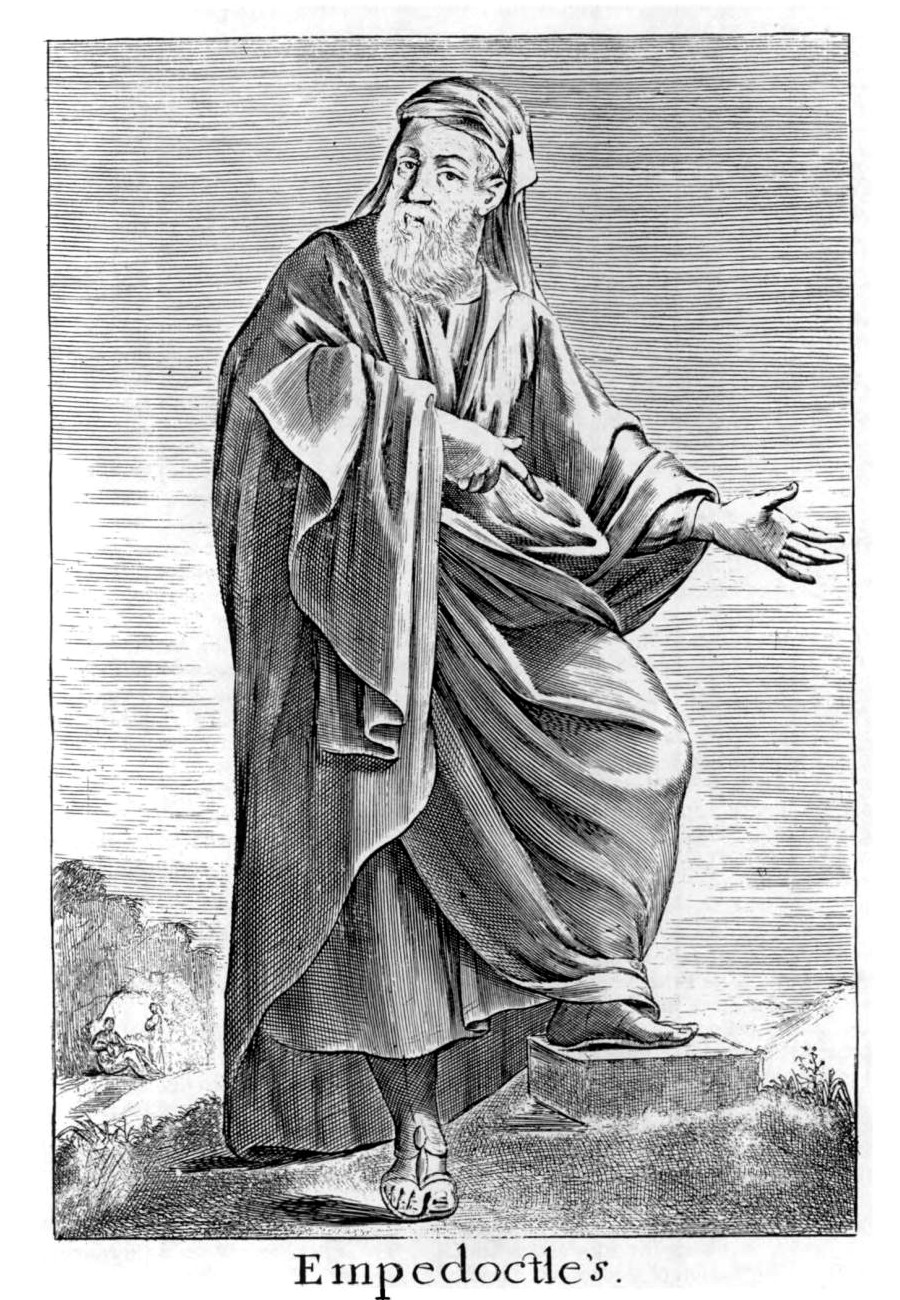
\includegraphics[width=0.4\linewidth]{../Chapter2/fig/empedocles.jpg}
		\caption{Empedocles~\cite{Stanley1655}}
		\label{fig:empedocles}
	\end{subfigure}%
	\begin{subfigure}{0.5\textwidth}
		\centering
		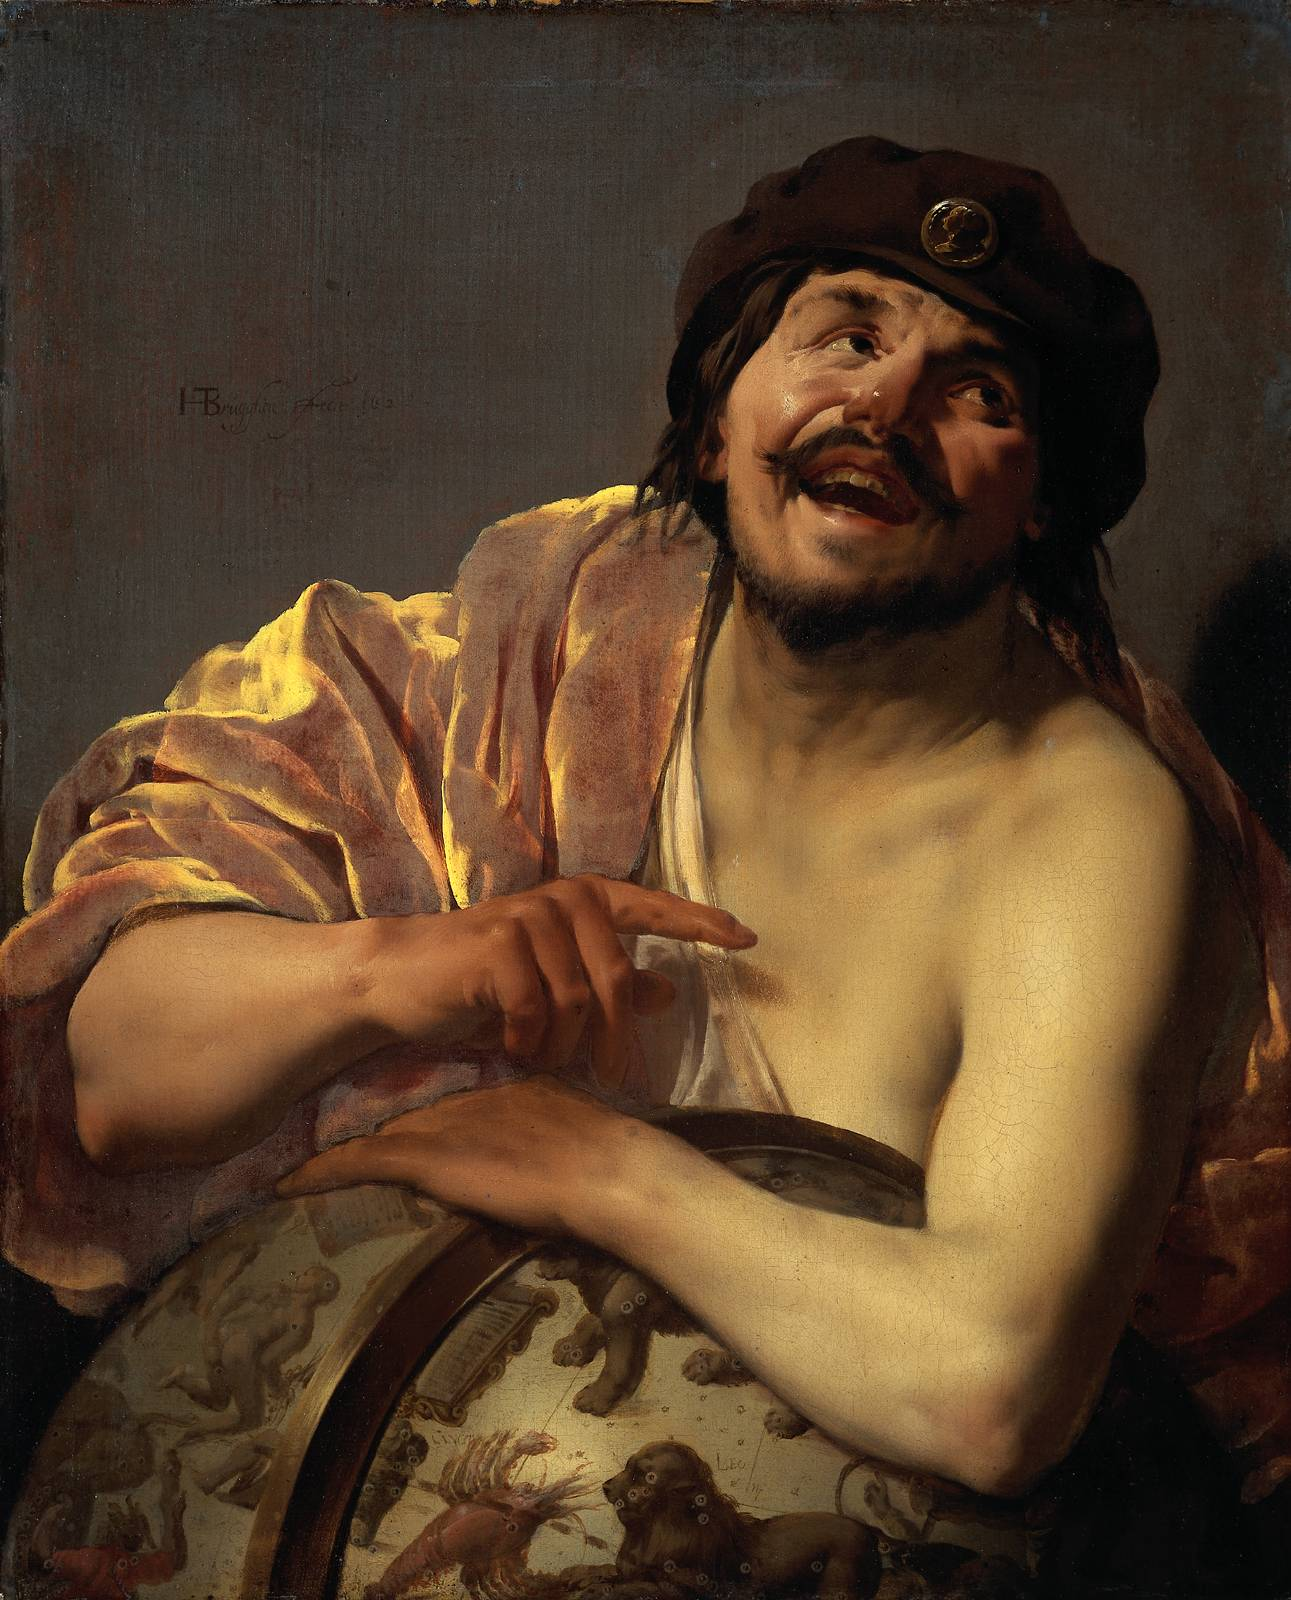
\includegraphics[width=0.4\linewidth]{../Chapter2/fig/democritus.jpg}
		\caption{Democritus~\cite{Brugghen1628}}
		\label{fig:democritus}
	\end{subfigure}
	\caption{ Two Greek philosophers, who made important philosophical
		contributions our understanding of matter. Empedocles (left), postulated the
		precursor to the elemental theory of matter ~\needcite{} and Democritus
		(right), postulated the precursor to the atomic theory of matter.  }
	\label{fig:atomists}
\end{figure}

Democritus was part of a movement of thought which was first to make the
intellectual jump that perhaps matter was not a continuum, but instead, composed
of 'atomon', small, indivisible particles which when configured together, created
all that is observable ~\needcite{}. Empedocles was making equally important
philosophical strides - in a manner complimentary to Democritus' opinion that
matter must be made of atomon, Empedocles argued that matter is composed of
elemental primitives ~\needcite{}.

Although Empedocles' 'periodic table' was only composed of Earth, Water, Fire,
and Air, the idea that some unseen transmutation of elemental forces might
generate observables in nature with quite different (but perhaps reminiscent)
properties then the 'pure substances' was an important step forward.
Proto-scientists were beginning to generate models which derived our complicated
observations, from simpler forms.

It took centuries of cultivation, leading up to the Scientific Revolution, for
the next great steps to occur, for science. Thankfully, the luminaries of the
Islamic Golden Age kept the fires of inquiry burning ~\needcite{}.

\clearpage
\subsection{The Scientific Revolution}

Thanks to the mathematical foundations laid out, build, and maintained by the
minds of the Islamic Golden Age, Europe was well poised to reignite the flames
of scientific inquiry, during the post Renaissance Scientific Revolution
~\needcite{}.

This period of growth in science was unprecedented during the Scientific
Revolution, thanks to the seeds of empiricism germinated during the Islamic
Golden Age, fertilized by the Italian Renaissance, and helped to flourish
through British Empiricism ~\needcite{}.

\begin{figure}[ht]
	\centering
	\begin{subfigure}{.5\textwidth}
		\centering
		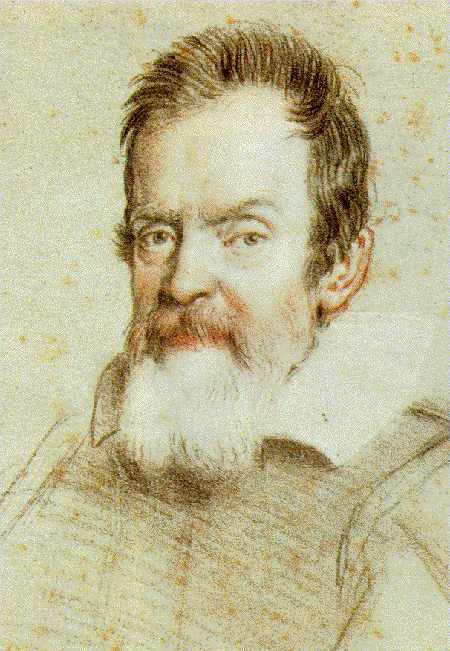
\includegraphics[width=0.4\linewidth]{../Chapter2/fig/galileo.jpg}
		\caption{Galileo~\cite{Leoni1624}}
		\label{fig:galileo}
	\end{subfigure}%
	\begin{subfigure}{0.5\textwidth}
		\centering
		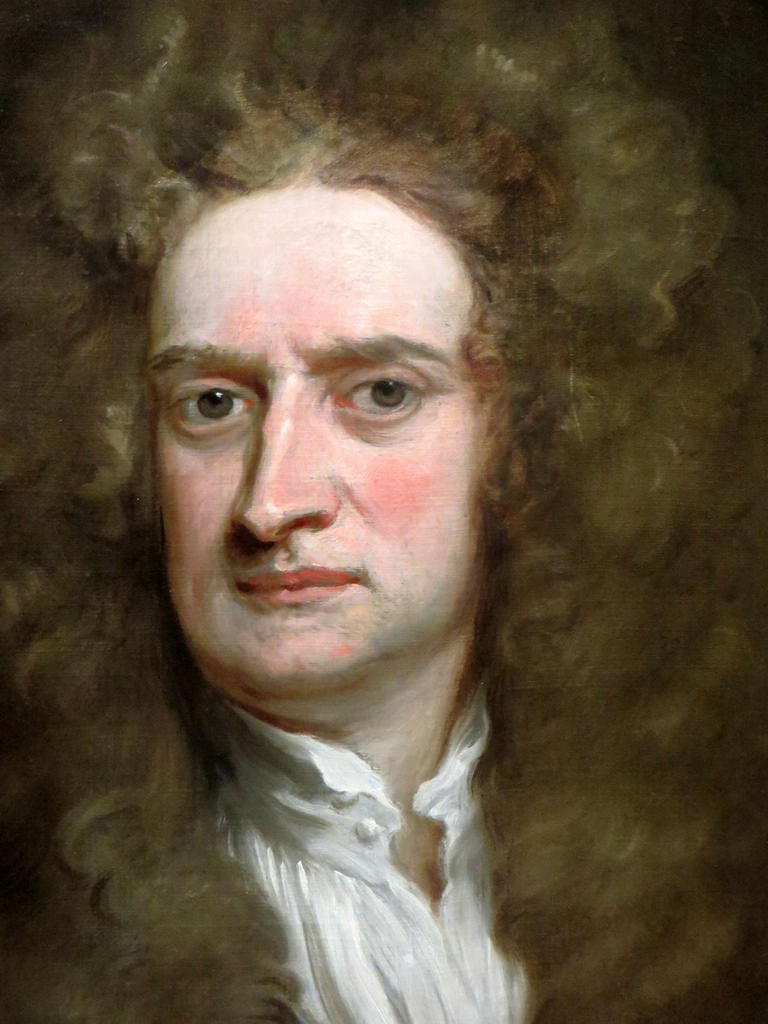
\includegraphics[width=0.4\linewidth]{../Chapter2/fig/newton.jpg}
		\caption{Newton}
		\label{fig:newton}
	\end{subfigure}
	\caption{ 
		Giants in the age of Empiricism, Newton (left) and
		Galileo (right) both made foundational contributions to Physics.
		Galileo lived in Italy, born in 1564 and dying in 1642. Newton lived in
		England from 1642 until his death in 1727
	}
	\label{fig:newtongalileo}
\end{figure}

\subsubsection{Galileo Galilei}
While Galileo is best known for his work in Observational Astronomy, his
importance to science extends beyond this. During his years in exile for his
controversial views of the heliocentric universe, he produced some of his most
important scientific work in kinematics ~\needcite{}. What made this work
remarkable is the care that Galileo took in merging careful mathematical
modeling with well designed experimentation. This methodical approach to inquiry
laid the foundation for others to slowly begin to pull back the curtains
obscuring physical law.

Galileo's formalization of the scientific method inexorably set science on a
course to delving deep into the nature of matter, and the laws of nature.

\subsubsection{Isaac Newton}
Fittingly born in the same year as Galileo's death, Isaac Newton would carry on
Galileo's legacy of rigorous mathematical modeling mixed with experimentation.
Perhaps no other scientist has touched so many different aspects of physics,
from theories of propagation of light, to celestial mechanics, to mathematics,
and kinematics.

Newton's Principia is perhaps the most important scientific work ever published.
It opened the doors of the universe in a way that nobody has since duplicated.
Newtons' laws of motion are still taught in school today, and although they have
since been shown to be inaccurate at the smallest and largest scales, they still
provide startlingly accurate predictions for the regular motion of matter.

One particularly tantalizing theory of Newton's was the corpuscular theory of
light. Although not his most influential theory by far, the idea that an
apparently continuous medium such as a beam of light might be made of small
packets of energy (corpuscles) turned out to be partially right ~\needcite{}.

Newton's theories, and contributions to science are enormous, and have moved us
deeper still into the underpinnings of matter. It would not be until roughly 200
years after his death, in the 19th century, that we finally can take the first
steps into the world of the atomic, and sub-atomic: the world of the proton. 

\clearpage
\subsection{Atomic Theory}

On the shoulders of giants such as Newton and Galileo, science finally came to
know the tool which has been indispensable to modern particle physics:
scattering. Rutherford and Thompson both carried out the most important
scattering experiments in modern science, and provided us with the first hints
of a hidden, quantum world, though it would not be until the 20th century that
these important experiments would be fully contextualized with a theory of
quantum scattering.

Scattering experiments offer a very powerful method where we one uses a well
known initial state of matter (typically in the form of a beam), allows this
beam to interact with an unknown configuration of matter, and measures the
scattered beam. By carefully studying the kinematics of the scattered beam, we
can create models which allow us to understand the structure of the target
matter or describe the nature of the interaction between the beam and target. 

\begin{figure}[ht]
	\centering
	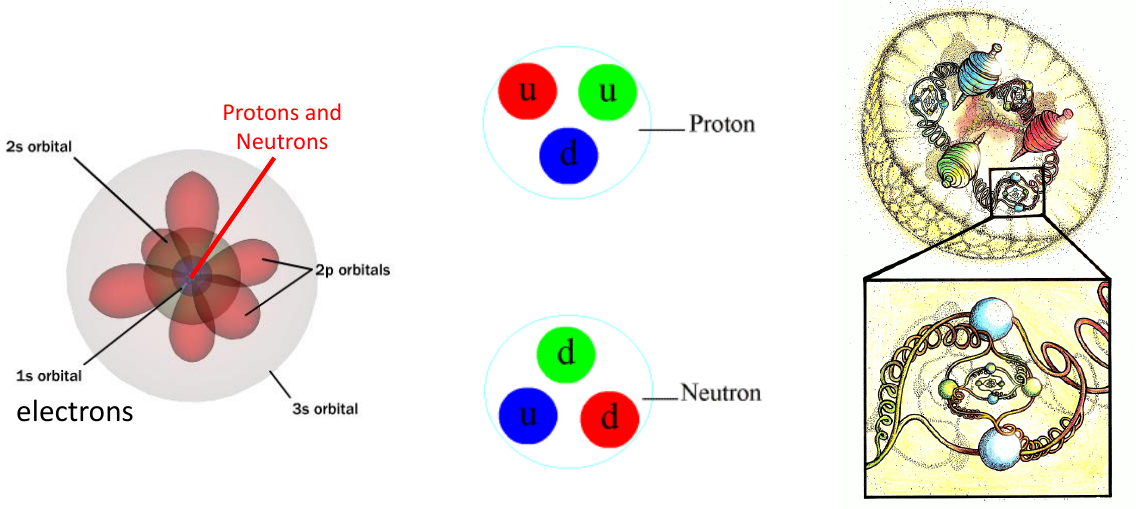
\includegraphics[width=\linewidth]{../Chapter2/fig/scale_of_matter.png}
	\caption{
		As we journey down further in scale, matter begins to look quite different.
		In fact, the models we use are scale dependent.
		Thomson~\ref{fig:thomsonrays}, and Rutherford~\ref{fig:rutherford} began to
		see matter as collections of atoms (left) ~\cite{Freudenrich2001} (though
		not in terms of the orbital structure pictured), though it would not be
		until 20th century quantum mechanics that electron orbitals were
		discovered.  Soon, nuclei were discovered to be divisible into protons an
		neutrons ~\cite{Manisearth2010} (center), which in turn were discovered to
		be composed of a sea of quarks and gluons (right). (Right image drawn by
		the talented Astrid Morreale, PhD, ~\cite{Morreale2009})
	}
	\label{fig:scale_of_matter}
\end{figure}

\subsubsection{John Dalton}

While many had postulated the existence of atoms, the first evidence based
theory which suggested the existence of atoms was produced by John Dalton in the
early 19th century. Dalton made an important conceptual leap to relate the
existence of stoichiometric ratios in chemistry to the presence of small,
individual functional units in his experiments with chemical reactions.
Dalton's realization was only made possible due to his careful accounting of
reactants in his experiments.

It was not until Einstein's 1905 theory on Brownian Motion was experimentally
verified by Jean Perrin to place limits on the mass and size of atoms that
Dalton's atomic theory was ultimately vindicated~\cite{Patterson200750}.

\subsubsection{J.J. Thompson}

\begin{figure}[ht]
	\centering
	\begin{subfigure}{.4\textwidth}
		\centering
		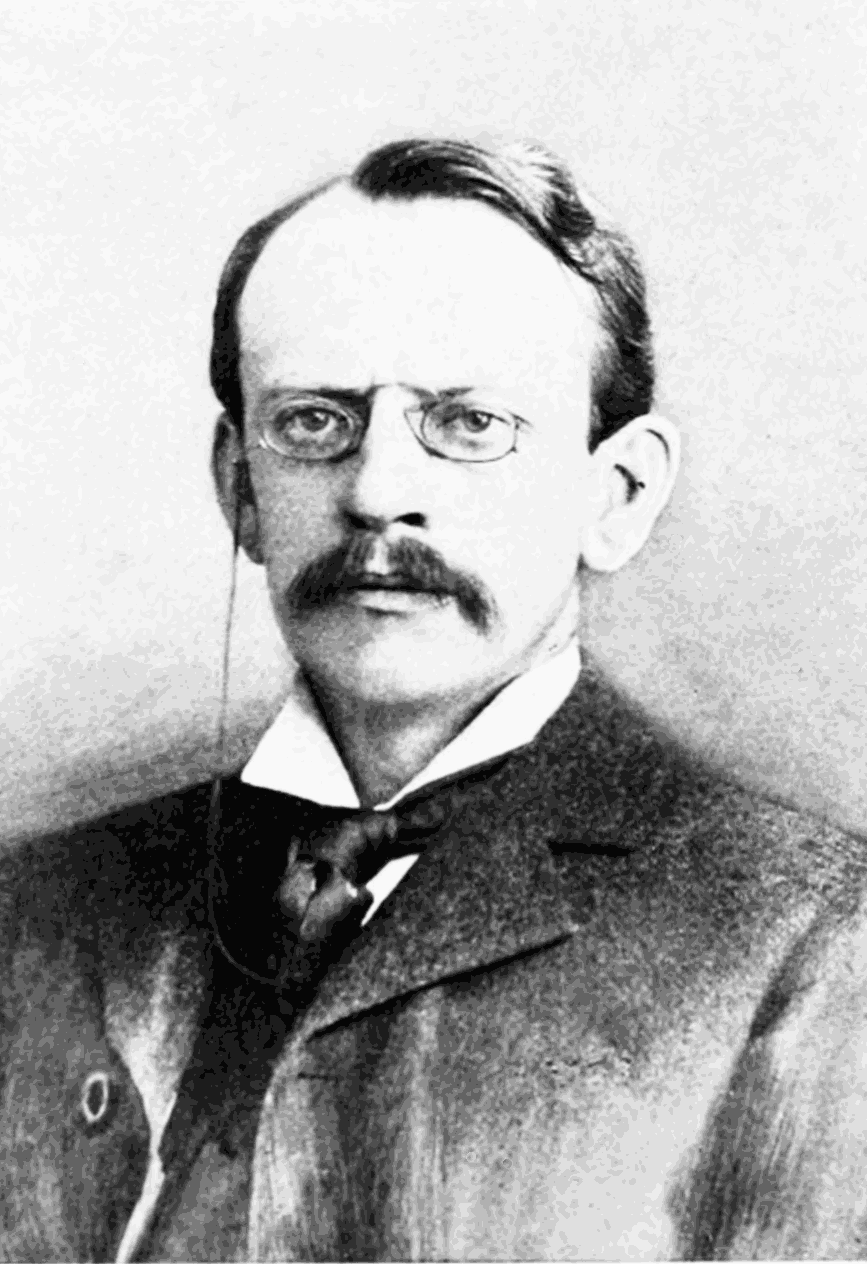
\includegraphics[width=0.4\linewidth]{../Chapter2/fig/jjthomson.png}
		\caption{J.J. Thomson ~\cite{PopularScience1899}}
		\label{fig:thomsonportrait}
	\end{subfigure}%
	\begin{subfigure}{0.6\textwidth}
		\centering
		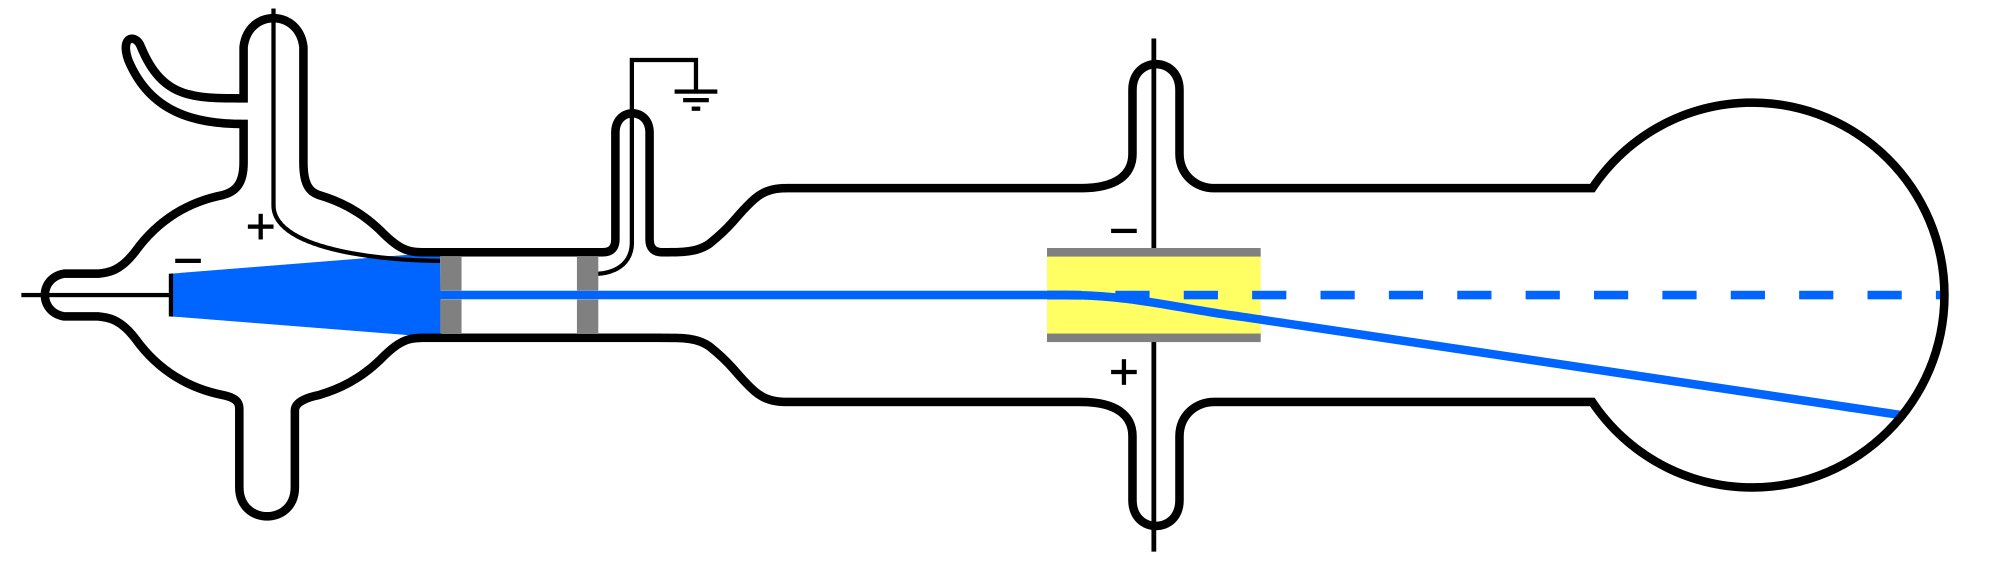
\includegraphics[width=0.4\linewidth]{../Chapter2/fig/cathoderaytube.png}
		\caption{Cathode Ray Tube ~\cite{Kurzon2010}}
		\label{fig:thomsoncathode}
	\end{subfigure}
	\caption{ 
		Left: J.J. Thomson, who showed that cathode ray tubes were in fact producing
		the first observed subatomic particle: the electron. Right: A cartoon of
		Thomson's cathode ray tube setup. Electrons would be deflected by a magnetic
		field, sent from cathode to anode.
	}
	\label{fig:jjthomson}
\end{figure}

Thomson (Figure~\ref{fig:jjthomson}) would discover that atoms are not the
smallest, indivisible piece of matter. In his landmark experiment, he used
cathode ray scattering experiments to show that cathode rays were in fact
subatomic particles. He showed these cathode rays were identical to particles
given off by the photoelectric effect, and that these same particles were
responsible for electric current. He had discovered the electron. And, if atoms
were not the smallest piece of matter, then perhaps, atoms themselves might not
be 'indivisible' as previously thought~\cite{nobelthomson2014}.

\subsubsection{Ernest Rutherford}

\begin{figure}[ht]
	\centering
	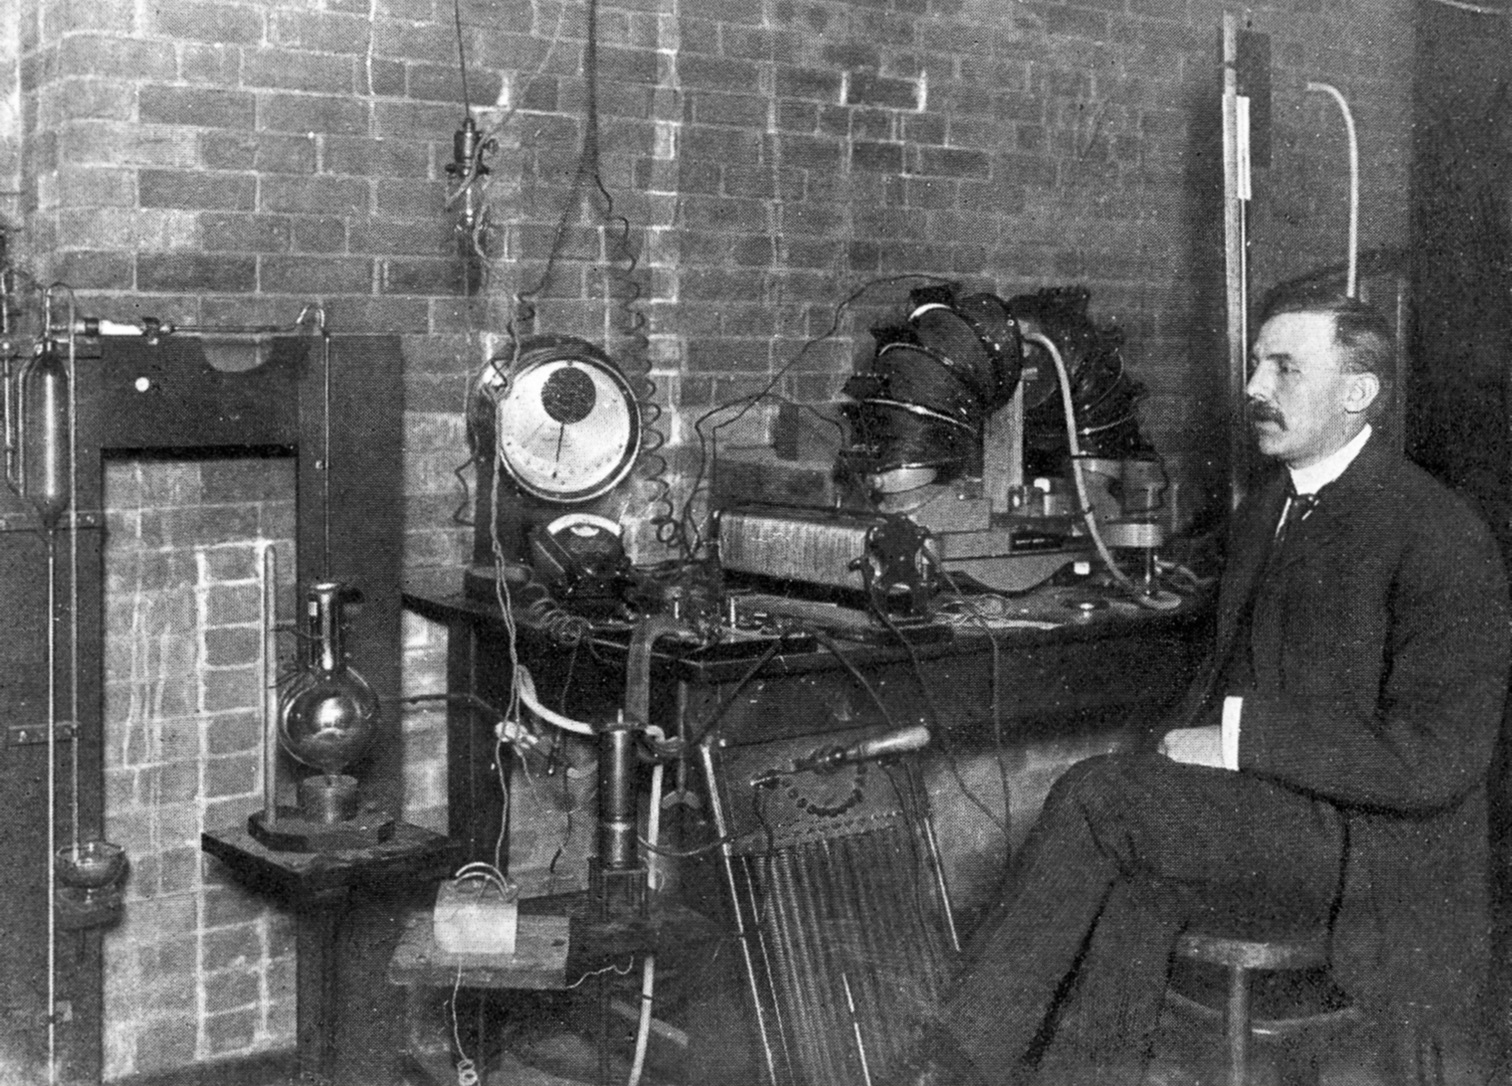
\includegraphics[width=0.6\linewidth]{../Chapter2/fig/ernestrutherford.jpg}
	\caption{Ernest Rutherford, in his lab. ~\cite{Eve1939}}
	\label{fig:rutherford}
\end{figure}

Ernest Rutherford (Fig~\ref{fig:rutherford}) was the first to show that atoms
themselves were highly structured - and consisted of a small dense center, later
called the nucleus.

\begin{figure}[ht]
	\centering
	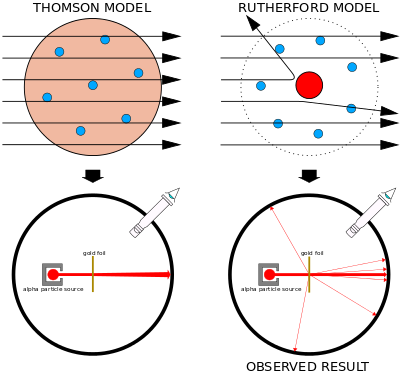
\includegraphics[width=0.6\linewidth]{../Chapter2/fig/geiger_marsden.png}
	\caption{
		Ernest Rutherford's historic experiment, showing (top right) that atoms were
		composed of a small dense nucleus, in contrast to Thomson's 'pudding model'
		of homogeneous charge (top left). The experiment, (bottom left and right)
		contrast the expected results (bottom left) against the observed results
		(bottom right) ~\cite{Kurzon2014}.
	}
	\label{fig:geigermarsden}
\end{figure}

Rutherford's work with radioactivity was of fundamental importance, he
discovered and classified both alpha-particle radioactivity and beta-particle
radioactivity. Further studies into these types of nuclear radiation would
unlock the nucleus of atoms through the work of future scientists. Notably,
Rutherford discovered the proton.

Rutherford's proposed planetary model for the nucleus, while technically wrong,
shifted paradigms from the pudding model of  atoms, to the more familiar nucleus
+ electron cloud model which has been spectacularly modeled and verified with
the forthcoming scientists which defined the field of quantum mechanics.

Rutherford's work helped push us our of the cocoon of classical mechanics into
the weird world of the quantum mechanics - scientists would soon find that the
nucleus is not just a dense concentration of charge, but a probabilistic
structure, with rich sub nuclear structure.

\clearpage
\subsection{Early Quantum Theory}

During Rutherford's time, experiments were already underway which were
investigating modeling light as a wave phenomena. This was in contrast to
Newton's (unverified) corpuscular theory of light. The argument whether light
was wave-like or particle-like eventually lead to a classical field theory
describing light, and the electromagnetic interaction, yet scientist such as Max
Plank were proposing theories which required the quantization of light.
~\needcite{}. Einstein would show that in his analysis of the photoelectric
effect, that light indeed was quantized into 'corpuscles'. The nascent atomic
theory of matter was also hinting at a hidden, quantized world.

\begin{figure}
	\centering
	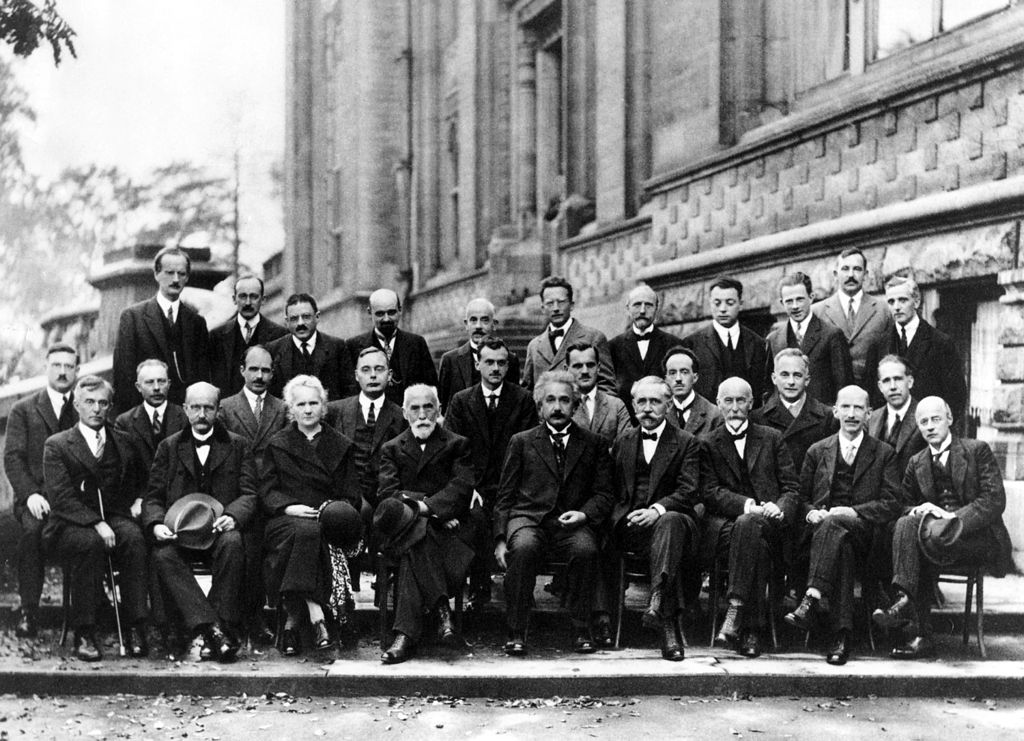
\includegraphics[width=\linewidth]{../Chapter2/fig/solvay.jpg}
	\caption{
		The attendees of the Solvay Conference in Brussels, 1927
	~\cite{BenjaminCroupie1927}.
	}
	\label{fig:solvay}
\end{figure}

At the Solvay Conference in Brussels, Figure~\ref{fig:solvay}, in 1927, we saw
an unprecedented gathering of some of the most important figures in modern
physics, all in one place, laying down the foundations of what would become
quantum mechanics. These scientists defined the nature and rules of quantum
mechanics - the weird model which accommodates a duality of matter - both
wave-like, and particle like. The notion that probing the structure of matter
did not yield a simple, deterministic hierarchy of structure was revolutionary,
confusing, and bizarre, and still is to this day.

It was found that not only light possesses this wave-particle duality, but also
the very particles that make up atoms as well. These models were formalized by
Dirac, Hilbert and Von-Neumann ~\needcite{}.

Though experiment tended to lead theory, regarding understanding the composition
and rules of interactions in matter, in the mid 20th century, further
refinements and additions to quantum mechanics gave birth to quantum field
theory. While early quantum models were very successful at describing static
particles trapped in static potentials - such as refining atomic theory to
include predictions of observed atomic spectra, more work was needed to
understand the relationship between electrical currents, light and magnetism.
These concepts were all related by Maxwell ~\needcite{} in the latter half of
the 19th century, but did not make good predictions for systems in motion.

Dirac was first to create a model for describing the electron, its behavior in
electromagnetic fields, and photon emission and absorption, under fully
relativistic and quantum conditions~\needcite{}. Dirac's model was so
successful, that it would become the basis for what we now call quantum
electrodynamics. Much of the mathematical formalism has been reused to describe
other field theories, which are the ultimate language which model and describe
the structure of matter - including the insides of a proton. 

\begin{figure}[ht]
	\centering
	\begin{subfigure}{.4\textwidth}
		\centering
		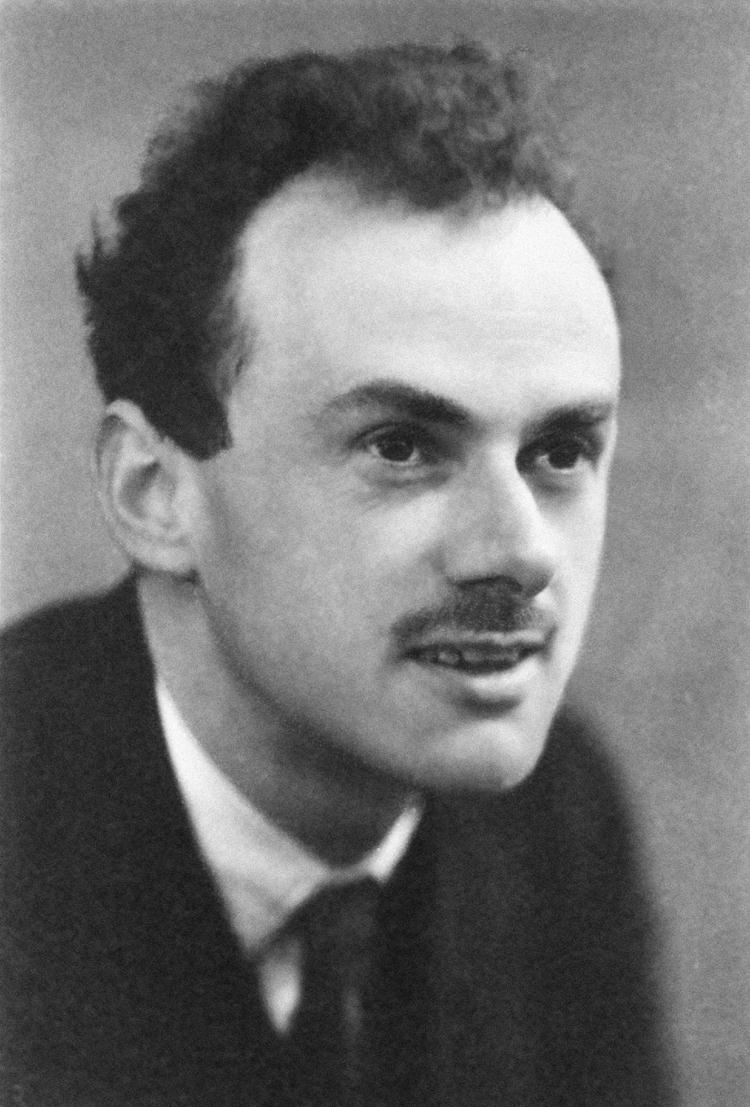
\includegraphics[width=0.4\linewidth]{../Chapter2/fig/pauldirac.jpg}
		\caption{Paul Dirac, 1933 ~\cite{NobelFoundation1933}}
		\label{fig:pauldirac}
	\end{subfigure}%
	\begin{subfigure}{0.6\textwidth}
		\centering
		\begin{equation}
			\left(\beta mc^2 + c\left(\sum_{n \mathop =1}^{3}\alpha_n p_n\right)\right) \psi (x,t) = i \hbar \frac{\partial\psi(x,t) }{\partial t}
		\end{equation}
		\caption{The Dirac Equation}
		\label{eq:diracquation}
	\end{subfigure}
	\caption{ 
		Paul Dirac, next to his original formulation of the Dirac Equation,
		describing the wave function for an electron with rest-mass $m$, in terms of
		its spacetime coordinates.
	}
	\label{fig:thomsonrays}
\end{figure}

Dirac's work also began to incorporate relativistic effects in his wave
equations modeling the electron, as well as crucially incorporating the spin
(I.e. Dirac Spinors) of these particles, which were important for making precise
predictions for atomic spectra~\needcite{}.

By this time, the proton was already known to reside in the enigmatic nucleus of
atoms, however, attempts to use Quantum Electrodynamics to describe the state of
the nucleus failed - it was clear that there was a very strong force, holding
together the protons of a nucleus tightly - far in excess of the electromagnetic
repulsion felt by the positively charged particles. There was a completely
different coupling strength between this apparent strong nuclear force, and the
better known electromagnetic coupling. Further complicating an understanding of
the nucleus is the fact that as the length scale of probing decreases, the
energies probed increase, fundamentally making the nucleus a relativistic
object. Experimental physics would once again, forge ahead, in attempting to
understand the inner workings of the nucleus, in the time-honored tradition of
performing scattering experiments.

\clearpage
\subsection{Early Particle Physics and The Eightfold Way}

The hydrogen atom, and its spectra was well modeled with quantum mechanics by
the end of early 20th century, however attempts to study Helium were not as
successful ~\needcite{}. However, in 1932,  when Chadwick turned a beam of
helium particles (at that time only known as $\alpha$ particles) on a sample of
Beryllium, he observed that neutral, non-ionizing, penetrating radiation was
produced ~\cite{KraussParticleHistory}. Photons were ruled out as possible
candidates, leading to the discovery of the neutron. Protons and neutrons were
hypothesized by Heisenberg to both be the same state of a new conceptual
particle, the nucleon, ~\cite{Heisenberg1952}. In the same year, Anderson
discovered the positron. 

By 1934, Hideki Yukawa (Fig.~\ref{fig:hidekiyukawa}) had created an effective
field theory for interactions of 'elementary particles' (at this time, thought
to be protons and neutrons). He predicted the existence of mesons, and wrote
down an effective field theory which described how protons and neutrons bind
together in the nucleus~\cite{Yukawa1935}. 

Though non-relativistic quantum mechanics was mostly complete by 1934,
scientists were already hard at work incorporating relativistic corrections to
the theory. Experiments with cosmic rays soon revealed the existence of muons
and the first observation of mesons.

\begin{figure}[ht]
	\begin{center}
		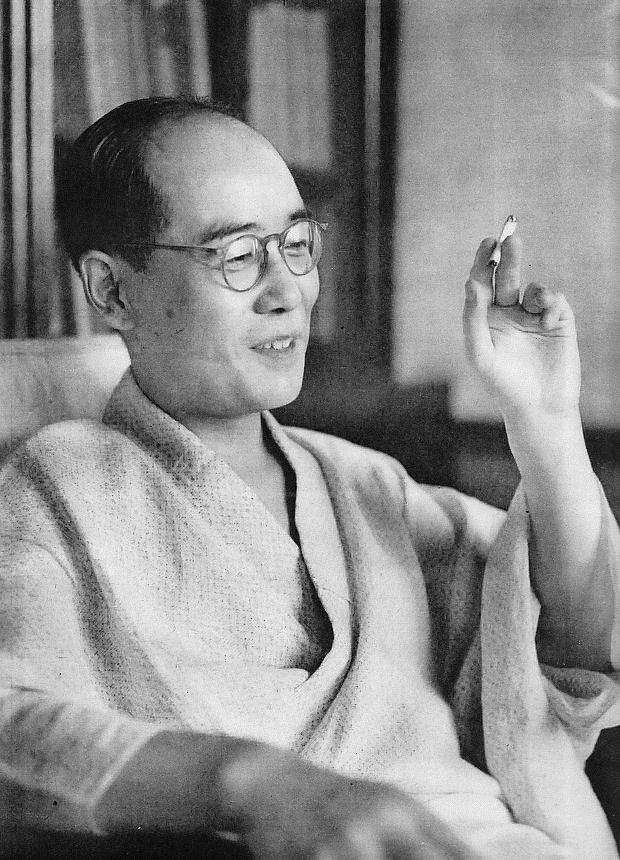
\includegraphics[width=0.5\linewidth]{../Chapter2/fig/hidekiyukawa.jpg}
	\caption{
		Hideki Yukawa, the first Japanese Nobel Laureate and publisher of influential
		research on the theory of mesons, and other elementary particles
		~\cite{YukawaPhoto1952}.
	}
	\label{fig:hidekiyukawa}
\end{center}
\end{figure}

Three separate paths eventually lead to the development of particle
accelerators, which are to date, the best mechanism we possess in physics to
probe nuclear structure. These accelerators are an outgrowth
of ever more intense Rutherford-style experiments, Tandem Van-Der-Graaf
generators, resonant acceleration techniques, RF linacs, and betatron
accelerators~\cite{Bryant1994}.

By the 1950's, a cornucopia of strange new particles had been discovered, both
matter and antimatter. But scientists drove forward, deeper, yearning to
discover what was fundamental. By the 50's, neutrinos had been proposed, as well
as Kaons, Pions, and Lambdas. Physicists were doing nuclear chemistry, in a
sense, attempting to work out how quickly some particles decayed, and what
decays were allowed or forbidden - science entered an age of nuclear alchemy.

"Strange" particles were discovered ($K$ and $\Lambda$), so called because in
bevatron experiments, they were produced in great quantities, but were slow to
decay, unlike the faster $\pi$ decay. Gell-Mann proposed that this strangeness
in matter was due to a new quantum number (he called it 'strangeness'). The name
stuck.
~\cite{Gell-Mann1953},~\cite{Gell-Mann1956},~\cite{KraussParticleHistory}.

The introduction of new conserved quantities, and the vast proliferation of
particles was in full swing - the subatomic world by the 1950's was confusing,
and complex. In his book "The God Particle", Leon Lederman recalled his adviser,
Enrico Fermi frustratedly remarking 'Young Man, if I could remember the names of
these particles, I would have been a botanist'. At this time, in the mid 1950's,
the number of mesons and baryons which had been discovered were at least in the
dozens, if not more.

While the use of particle accelerators were speeding us along in  our search for
the structure of matter, one particular invention truly revolutionized the
field - the bubble chamber (Figures~\ref{fig:bubble_chamber} and
~\ref{fig:bubble_tracks}.)

The bubble chamber was essentially a large vat of supercritical fluid which
could easily be caused to boil with small perturbations. This feature was
exploited, by positioning a bubble chamber in a magnetic field (to cause charged
tracks to bend) near the interaction point between a particle beam and a fixed
target. The bubble chamber itself was sometimes the target - since a popular
liquid to use was hydrogen. 

\begin{figure}[ht]
	\centering
	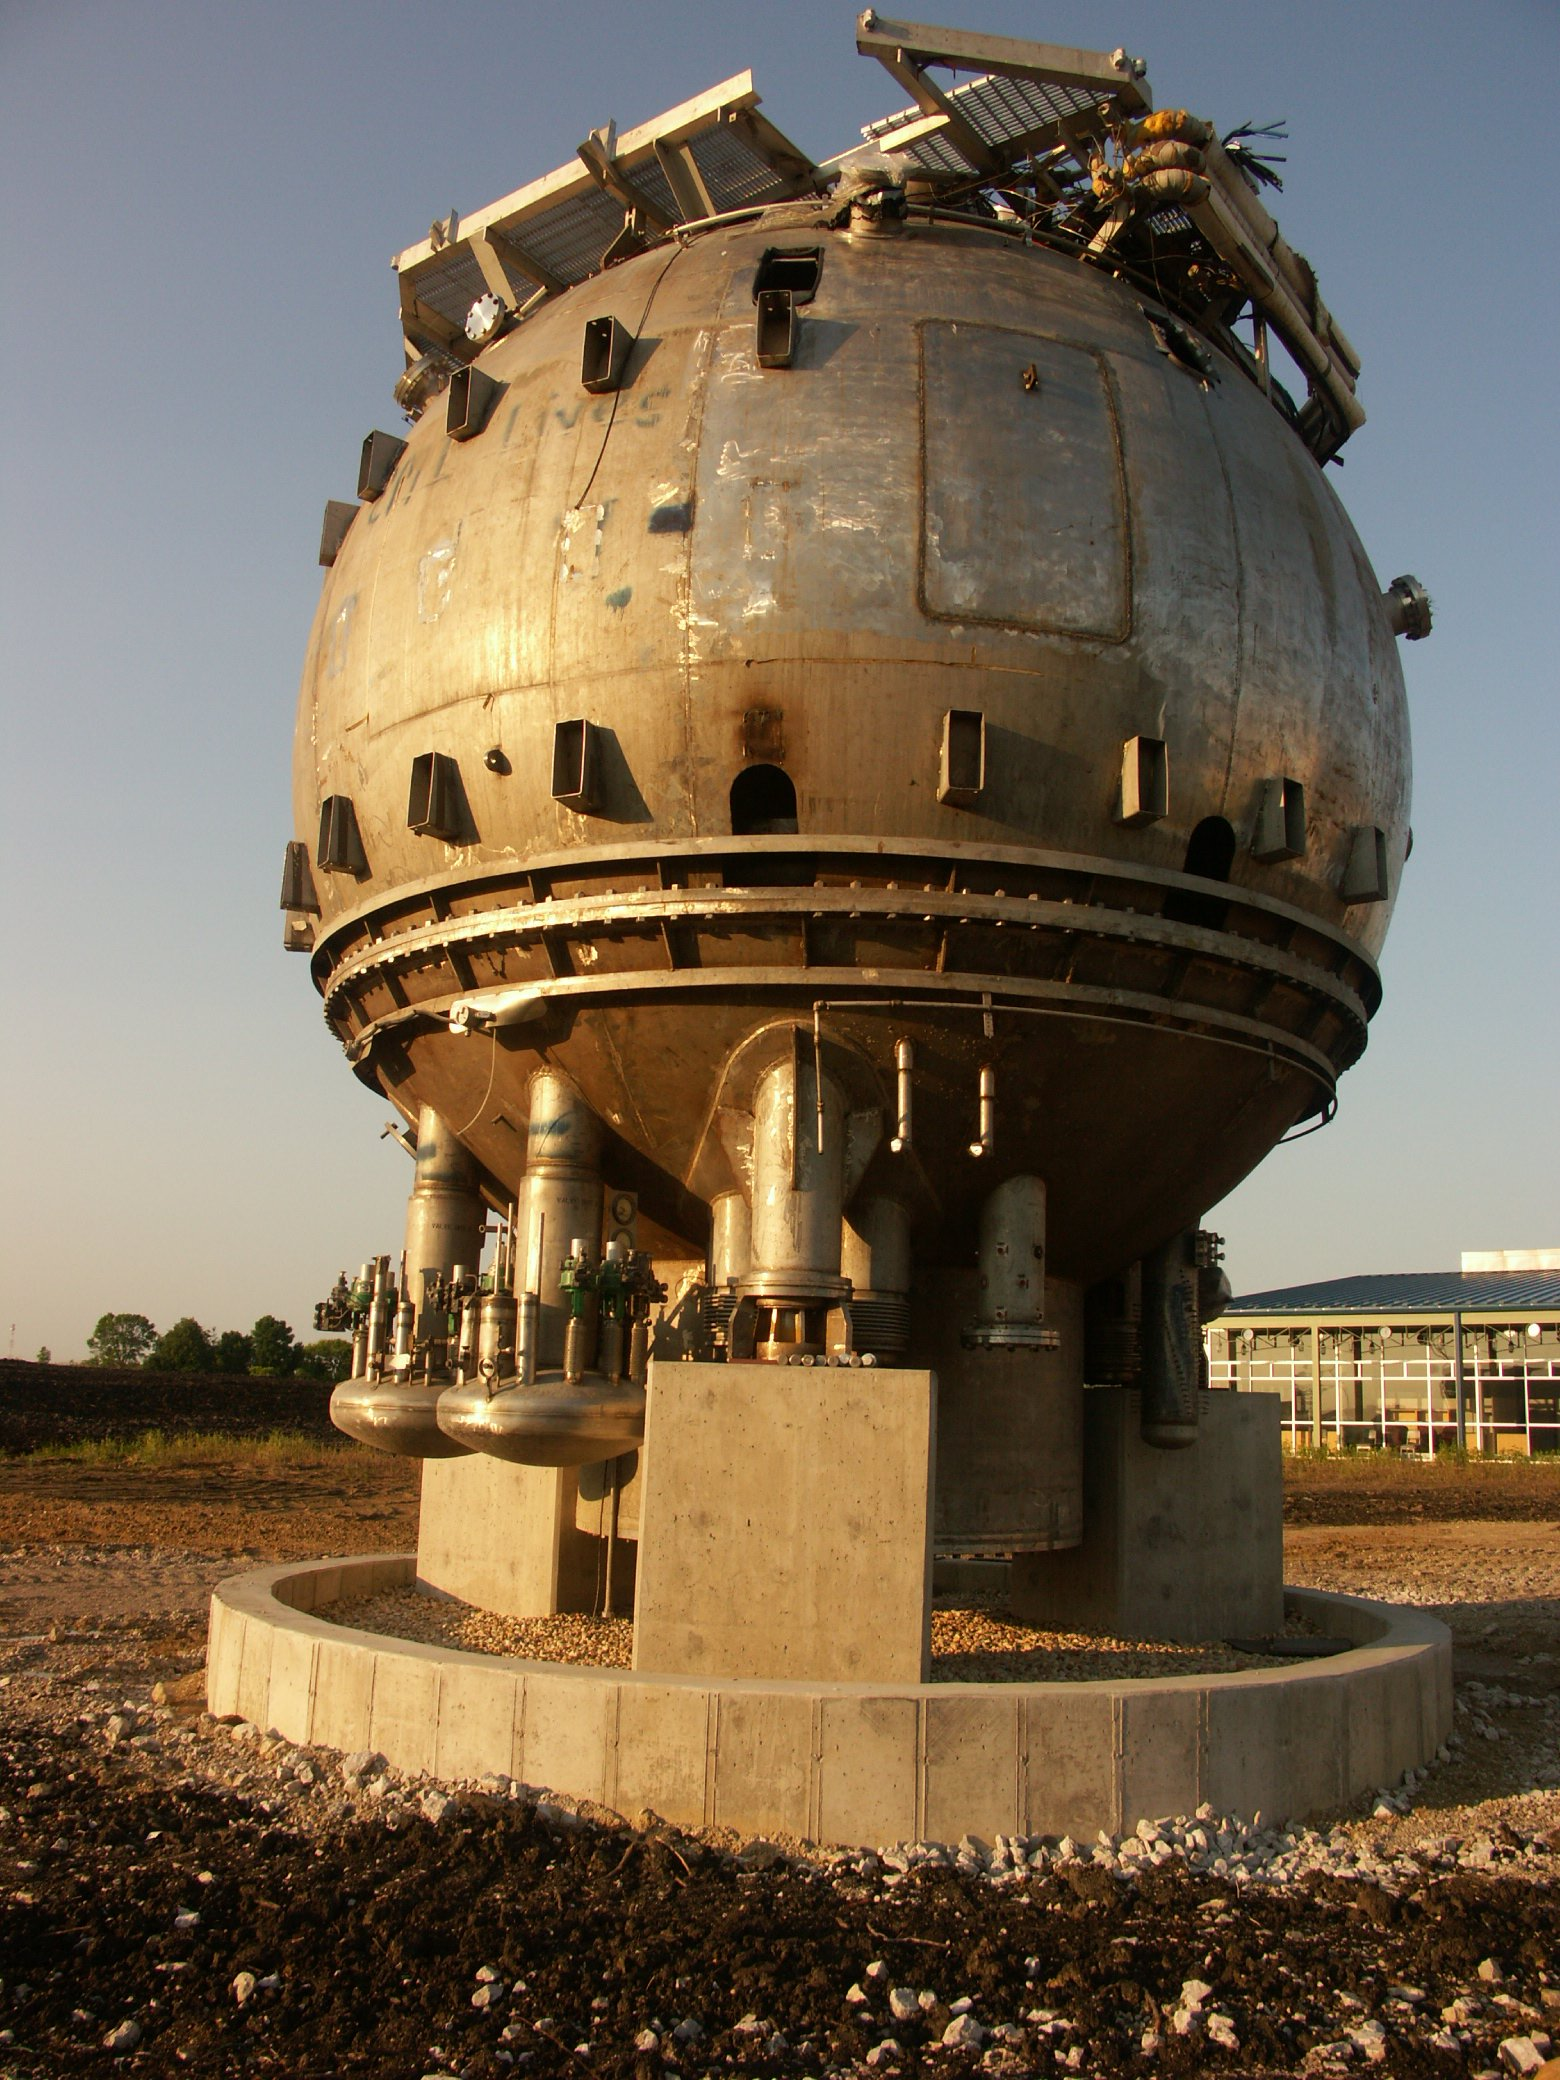
\includegraphics[width=0.5\linewidth]{../Chapter2/fig/bubblechamberfnal.jpg}
	\caption{An old bubble chamber, once used at Fermilab,
	~\cite{FNALBubbleChamber2005}}
	\label{fig:bubble_chamber}
\end{figure}

Invented by Donald Glaser in 1952, the bubble chamber was 'perfected' by Luis
Alvarez when he helped to develop a version which could be used with liquid
hydrogen. Hydrogen was desirable as a substance due to its extremely simple
structure, which supplied much cleaner results than other fillings, unlike the
original filler, Ether.

\begin{figure}[ht]
	\centering
	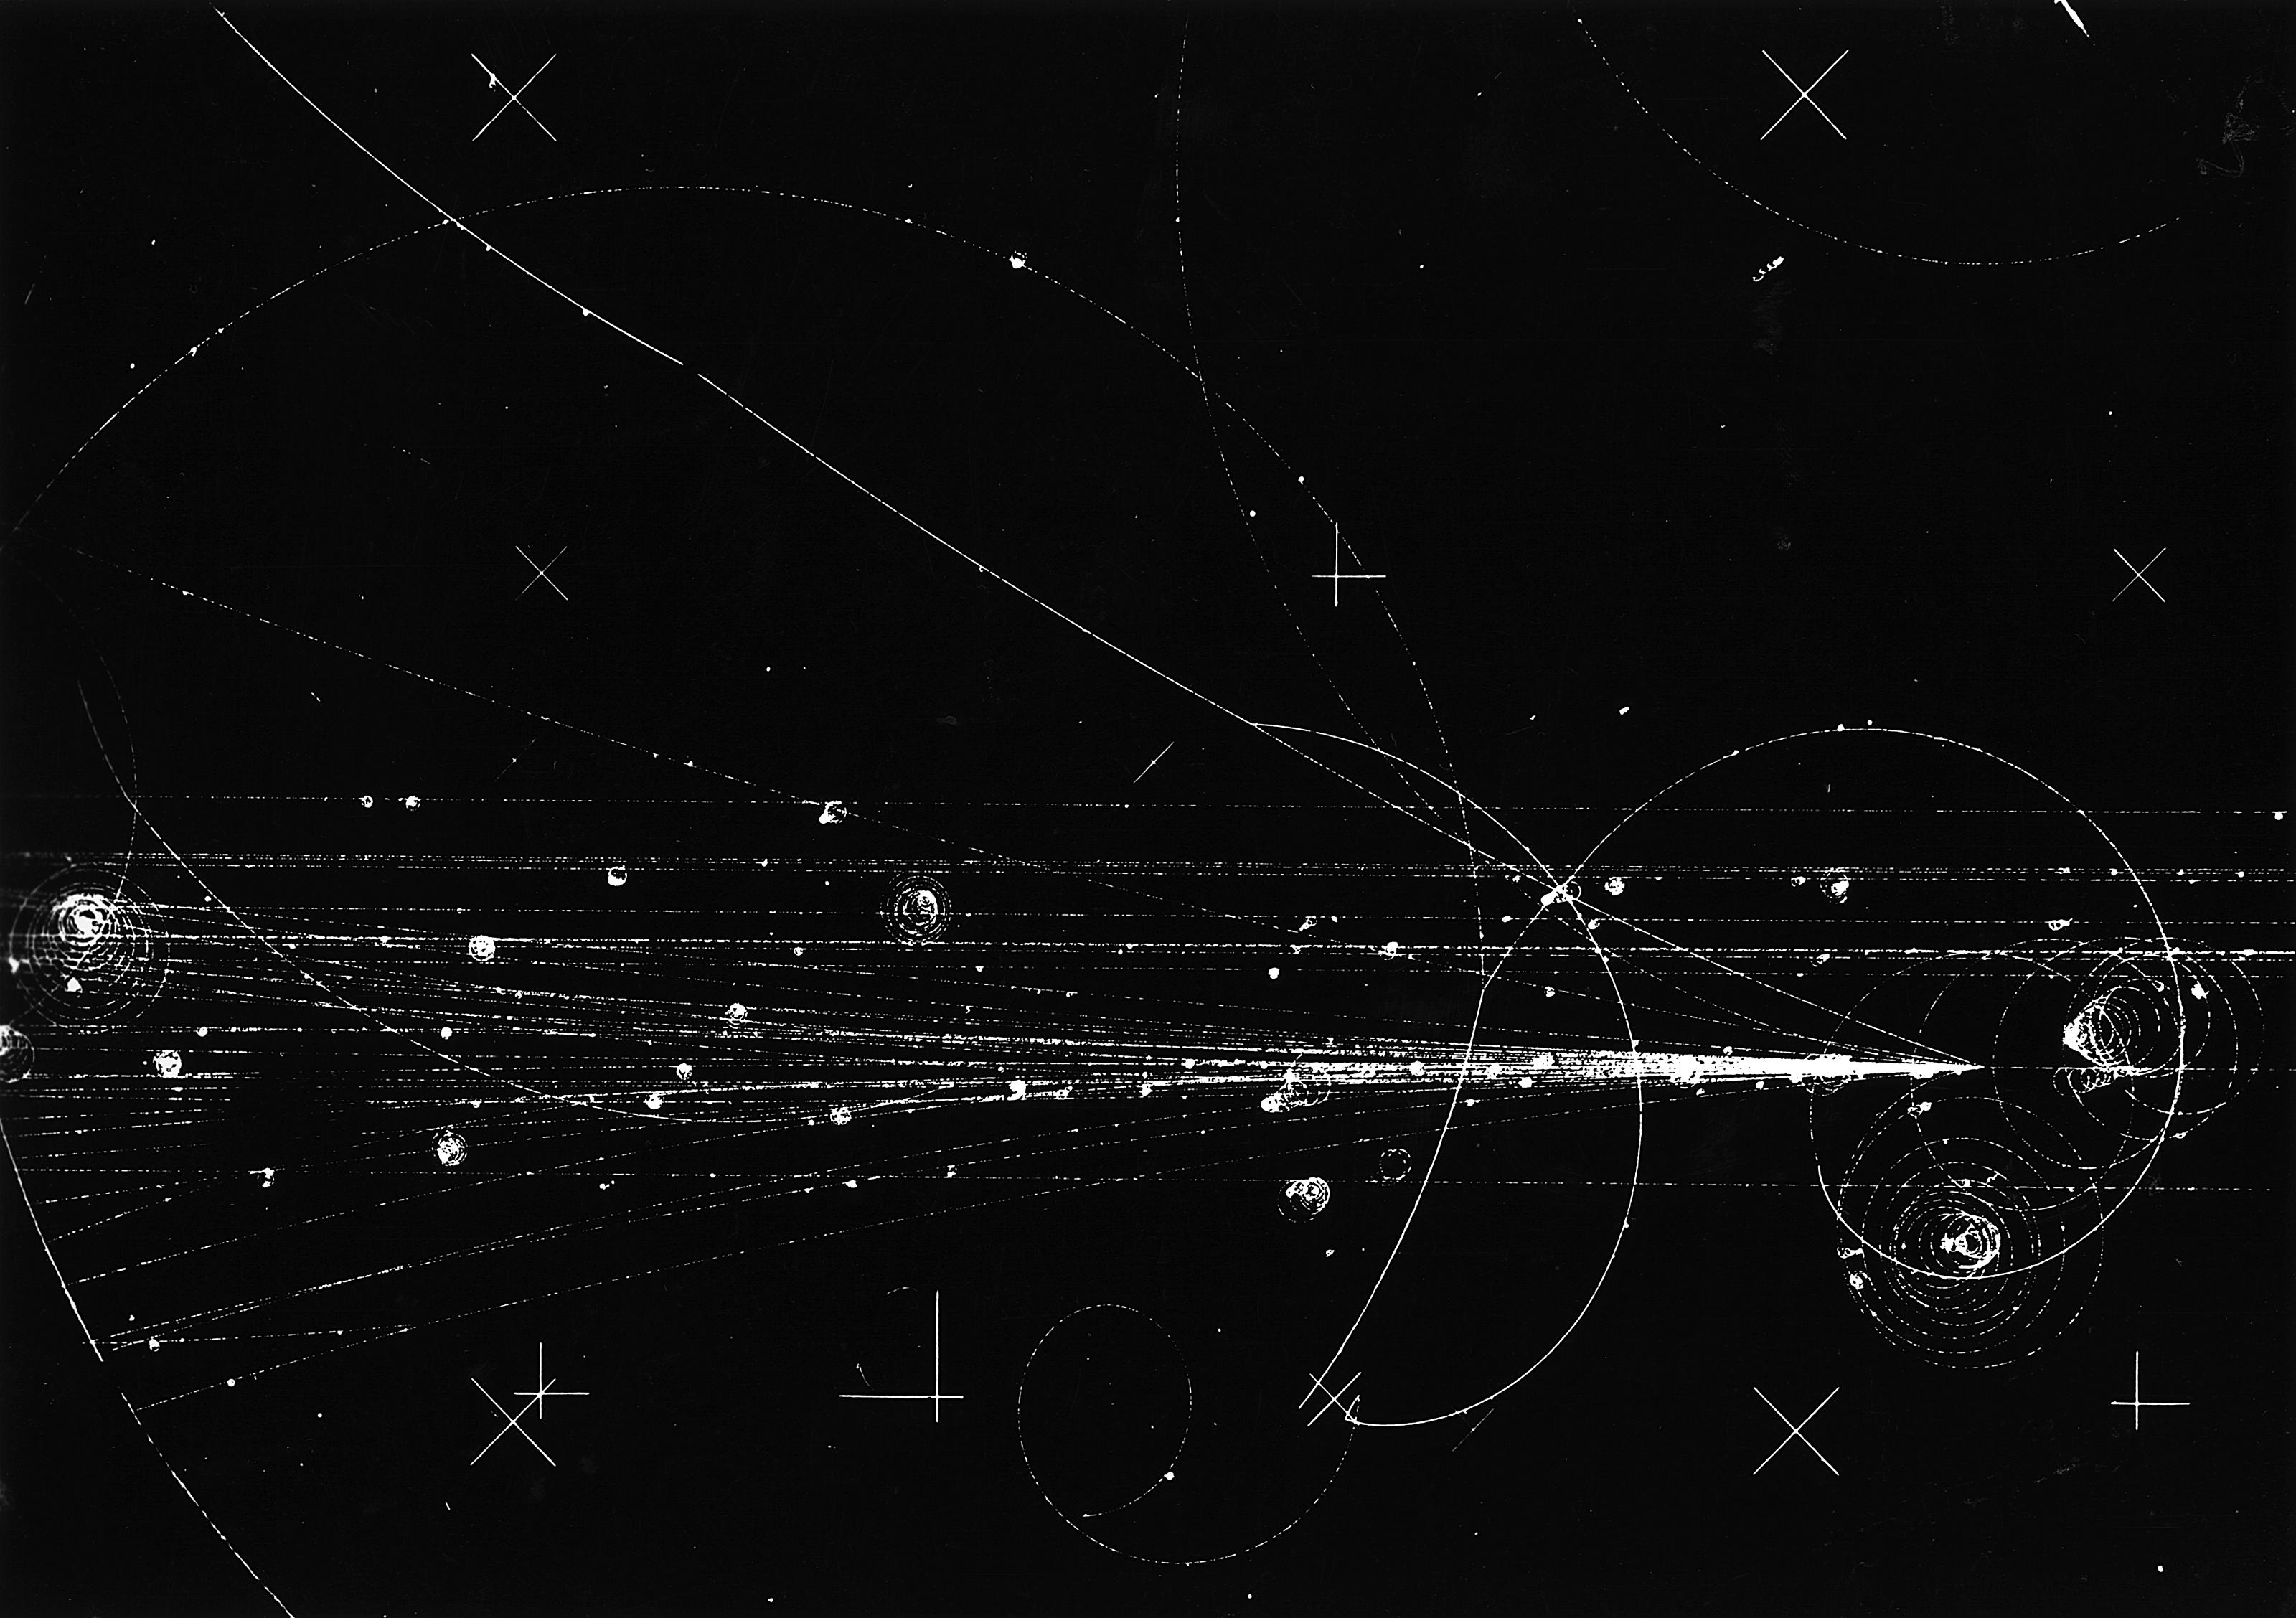
\includegraphics[width=0.5\linewidth]{../Chapter2/fig/bubble_chamber_tracks.jpg}
	\caption{
		An example of the photographs taken with a Bubble Chamber, in 1973.
		In this picture, we see a 300 $GeV$ proton producing partices as it travels
		through a hydrogen-filled bubble chamber at fermilab ~\cite{HD6B235}.
	}
	\label{fig:bubble_tracks}
\end{figure}

Soon after the advent of bubble chambers, physicists were able to
macroscopically image these new, exotic particles interacting with normal matter
as well as decaying - and develop novel computer techniques to analyze and
catalog the massive influx of data.

The break-through came in 1961, when Gell-Mann and Nishijima leveraged
recognized the underlying symmetry of the interactions taking place, and created
what would be known as 'the eightfold way'. This theory created a scheme for
organizing the observed baryons and mesons according to their properties in
groupings called "octets". These octets were in fact representations of the
elements of members of the $SU(3)$ group. Another way of stating this, is that
Gell-Mann had discovered the underlying structure of flavor-symmetry between the
three lightest quarks - $u$, $d$, and $s$. This work directly led to the
development of the quark model of matter, the foundation of what would become
the foundation of the standard model of particles. To date, the standard model
is the most successful theory describing particles, and their interactions.

Gell-Mann's quark model soon made important predictions which were later
verified, notably the $\Omega^{-}$, which was the ground-state particle of the
spin-$3/2$ decuplet - discovered at Brookhaven National Laboratory (the same lab
from which my research has been derived!). 

Gell-Mann formalized his quark theory of matter in 1964, however, due to the
unforeseen phenomena of color confinement, it would be several years before
evidence of quarks composing baryons and mesons was directly obtained from deep
inelastic scattering experiments.

\clearpage

\section{Deep Inelastic Scattering and The Parton Model}

Deep inelastic scattering experiments, Figure~\ref{fig:disschematic} were a natural
outgrowth of Rutherford's experiment from the late 19th century. There are a few
notable differences.  Rutherford's scattering experiments could be modeled
classically, by assuming some concentrated charge center to atoms, and using an
impact parameter for an incoming projectile to predict where projectiles were
scattered. Rutherford's experiments were considered generally 'elastic' because
the target absorbed very little kinetic energy from the projectile.

However, in the late 20th century, scattering experiments became highly
inelastic - targets would absorb a lot of kinetic energy - sometimes so much
that targets would be utterly destroyed. Inelastic scattering experiments don't
merely blow up our targets - otherwise there would be no point to undertake the
experiment in the first place. Instead, what happens in deep inelastic
scattering, is that during the process of a high energy interaction between the
projectile (often a beam) and the target (often an ionized gas, sometimes
another beam), some kind of interaction occurs between the target and the
projectile, in a way that changes the state of the projectile, and generates
matter due to the high energies involved. One can observe the state of the
projectile, and account for the matter which is created, and if there are laws
which govern how the state of the projectile changes, or the kinds of matter
that can be created, then we can run the clock backwards, reconstructing the
kind of interactions that happened, to learn something about nuclear structure
(or even partonic structure). In this way, one can also identify conserved
quantities, which in turn suggest physical symmetries, which in turn help to
build models.

I said the word parton, which I have been carefully avoiding, but now the cat's
out of the bag. Nuclei, as we will learn, are not elementary particles, but
instead, are built up from what we assume are fundamental, elementary particles.
Deep inelastic scattering experiments slowly revealed that nuclei (individual
protons and neutrons) were not elementary particles, but instead, composite
particles. It is natural to assume then, that the properties of protons and
neutrons are not fundamental either. And in fact, the vast zoo of particles that
were discovered in early inelastic scattering experiments, such as $\pi$ or $K$
or $\Lambda$ (discussed briefly earlier) were not fundamental either.

In Michael Riordan's excellent 1992 summary of the discovery of quarks, Riordan
lays out a very succinct and thorough history of the late 20th century
experimental and theoretical works which built on Rutherford and Gell-Man's
work. Riordan states that surprising 'results came from a
series of electron scattering experiments...from 1967 through 1973' at MIT and
SLAC, which comprised the first set of evidence produced in favor of the
partonic model. As described earlier, Gell-Mann created a three-quark model to
produce predictions consistent with these observations~\cite{Riordan1992}.

\begin{figure}
	\centering
	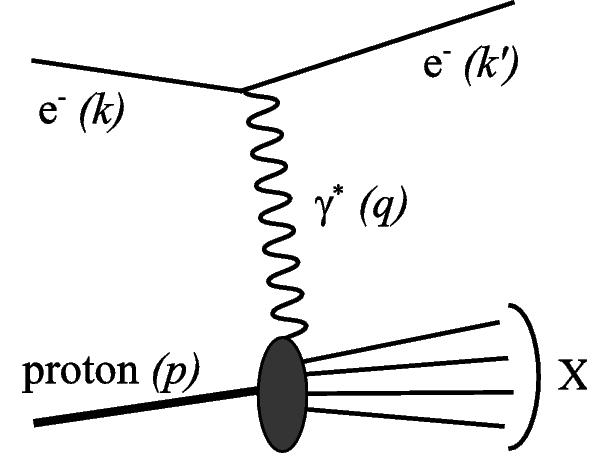
\includegraphics[width=0.6\linewidth]{../Chapter2/fig/deep_inelastic_basic.png}
	\caption{
		A schematic of deep inelastic scattering, where the incoming electron
		inelastically scatters off the proton, producing results $X$, via virtual
		photon exchange, $\gamma^*$ ~\cite{Ddn2_2008}
	}
	\label{fig:disschematic}
\end{figure}

By the 1970's, collaborations between Bjorken, Feynman, and others had produced a
coherent partonic model which contained quarks, and force mediating gluons.
Additionally, the concept of Structure functions had been developed. Modified
from Rutherford's original scattering formula, this new formula to describe the
cross section of deep inelastic scattering incorporated structure functions,
which separated out the momentum exchange between target and projectile (via a
virtual photon), and isolated this from $W_1$ and $W_2$, structure functions
which were experimentally measured quantities representing the electron-proton
interaction (the 'physics-y' part of the interaction).

EIC white paper: ~\cite{Accardi2012}

Discuss SLAC, CERN, DESY, and RHIC. Discuss although DESY took data with HERA
from 1992 - 2007, analysis and publication of the data is still ongoing.

HepData: \url{http://hepdata.cedar.ac.uk/review/f2/index.shtml}

\subsection{CERN - European Muon Collaboration: 1979-1997}
Overview Paper: Higlights of the European Muon Collaboration
~\cite{Kullander1990a}

Although Gell-Mann's simple quark model of baryons ~\cite{Gell-Mann1961}
predicts the correct quantity for the spin of the proton, the work of Ashman et
al (1988) ~\needcite{} at the European Muon Collaboration directly measured a
portion of the proton structure function $g_1$ and found that a rather small
fraction of the proton spin comes from quarks - and most of the spin is carried
by the gluons (Figure~\ref{fig:emc_g1_result}).

\begin{figure}[ht]
	\begin{center}
	
\includegraphics[width=0.5\linewidth]{../filler/squareimg.png}
	\caption{
		~\needfig{} ~\needcap{}. Results of EMC experiment showing that the structure
		function g1, tells us a thing about proton spin.
	}
	\label{fig:emc_g1_result}
\end{center}
\end{figure}

inSPIRE: collaboration:'European Muon'

\subsection{SLAC - E142: 1993-1994}
inSPIRE: collaboration:'E142'

\subsection{SLAC - E143: 1992-1999} 
inSPIRE: collaboration:'E143'

\subsection{DESY - ZEUS: 1992-Present}
inSPIRE: collaboration:'ZEUS'
H1+ZEUS combined results: \url{https://www.desy.de/h1zeus/combined_results/}
ZEUS figures: \url{http://www-zeus.desy.de/zeus_papers/zeus_papers.html}

\subsection{CERN - Spin Muon Collaboration: 1993-1998}
Spin Asymmetry $A_1$ and structure functions $g_1$~\cite{Adeva1998}
NLO QCD analysis of spin structure function $g_1$~\cite{Adeva1998a}
inSPIRE: collaboration:'Spin Muon'

\subsection{SLAC - E154: 1994-1997} 
inSPIRE: collaboration:'E154'

\subsection{DESY - HERMES: 1995-2007}
inSPIRE: collaboration:HERMES
HERMES website, publications, figures: \url{http://www-hermes.desy.de/}

\subsection{SLAC - E155: 1997-2003}
inSPIRE: collaboration:'E155'

\subsection{CERN - COMPASS: 2005-Present}
inSPIRE: collaboration:'COMPASS'

\subsection{DESY - H1: 1992-Present}
H1 Publications: \url{http://h1.desy.de/e104552/e104555/}
inSPIRE: collaboration:'HERA' (HERA is the accelerator)
inSPIRE: collaboration:'H1' (this is the data)


\chapter{Models and Associated Probes For Proton Spin Structure}
\section{ structure functions}
\section{ proton spin decomposition}
\section{ unpolarized parton distribution functions}
\section{ polarized parton distribution functions}
\section{ that sweet table from Delia hasch}
\section{ discussion $\bar{q}$, $q$, $L_q$, $g$}
\section{ DSSV }

\clearpage
\section{Measurement of the Proton Spin}
\subsection{ physics probes for proton spin}
\subsection{ W cross section}
\subsection{ derivation of Asymmetry}
\subsection{ kinematic extremes of Asymmetry}

\clearpage
\section{Cross Sections and Luminosity}
\begin{itemize}
		\item vernier analysis note intro, equations
		\item summarize the papers on Lumoninosity
\end{itemize}

\clearpage

\chapter{Experimental Apparatus}
\section{The Relativistic Heavy Ion Collider}
\subsection{Overview}
\subsection{The RHIC Spin Program}
\subsection{Production of Polarized Proton Beams}
\section{The Pioneering High Energy Nuclear Interaction Experiment}
\subsection{Subsystem Overview}
\subsection{Luminosity}
\subsection{Beam Polarization}
\section{The Forward Upgrade}
\subsection{The Muon Tracker + Muon Trigger Subsystems}
\subsection{Resisitive Plate Chambers}
\subsubsection{Design}
\subsubsection{Construction}
\subsubsection{Testing}
\subsubsection{Performance}
\subsection{The DAQ}
\subsubsection{2013 Data Set Triggers}

\chapter{The Data Set}
\label{ch:data_collection}
\section{Overview}
Now that we have discussed the various aparatuses provided by the PHENIX
experiment, we can go into more depth with the process of engineering features.
For this analysis, we consider only events which are identified by the Muon Arms
subsystem as being muons. The raw data provided by PHENIX is quite complex, and
at the hardware level is generally not too useful for physics analysis.

In this chapter, we will discuss the process of cleaning our data set, the goal
of which is to get rid of background data, while keeping any event that could
possibly contribute to the $W\rightarrow\mu$ signal. This cleaning is done in
three stages. The first stage concerns applying a simple basic cut to our data
set to remove events which are kinematically forbidden from having $W$ boson
parent particles, this is called the "Basic Cut".

After this, we label data with $W_{ness}$, which is an event's likelihood for
coming from a $W$ boson decay. Although this is part of data cleaning, since
$W_{ness}$ is an important parameter in the analysis, it is discussed in
Section~\ref{ssec:likelihood}.

Finally, we must estimate the overall yield of $\mu$ resulting from the various
proton helicity combinations, and the signal to background ratio characterizing
that yield. Again, since this is also an important part of the physics, it is
discussed in Section ~\ref{ssec:sbr}.

\section{Analysis Variables and the Basic Cut}

A brief summary of the kinematic variables used later in the analysis is given
in Table~\ref{tab:basic_cut}. In addition four sets of RPC cluster variables exist
which are being used as main RPC variables. These variables contain
projections from either vertex, Station 1, 3 or the MuID road to the
corresponding z positions of the RPCs based on the tracks in the PHMuoTracksOut
node and are directly taken over from the RpcMuoTracks node in the dsts:

\begin{itemize}
\item newsngmuons$\rightarrow$Branch("RpcMatchVtx",0,"Rpc3dca[\_RecoTracks]/F:\\Rpc3time[\_RecoTracks]/F:Rpc3x[\_RecoTracks]/F:Rpc3y[\_RecoTracks]/F:\\Rpc1dca[\_RecoTracks]/F:Rpc1time[\_RecoTracks]/F:Rpc1x[\_RecoTracks/F:\\Rpc1y[\_RecoTracks]/F");
\item newsngmuons$\rightarrow$Branch("RpcMatchSt1",0,"Rpc3dca[\_RecoTracks]/F:\\Rpc3time[\_RecoTracks]/F:Rpc3x[\_RecoTracks]/F:Rpc3y[\_RecoTracks]/F:\\Rpc1dca[\_RecoTracks]/F:Rpc1time[\_RecoTracks]/F:Rpc1x[\_RecoTracks]/F:\\Rpc1y[\_RecoTracks]/F");
\item newsngmuons$\rightarrow$Branch("RpcMatchSt3",0,"Rpc3dca[\_RecoTracks]/F:\\Rpc3time[\_RecoTracks]/F:Rpc3x[\_RecoTracks]/F:Rpc3y[\_RecoTracks]/F:\\Rpc1dca[\_RecoTracks]/F:Rpc1time[\_RecoTracks]/F:Rpc1x[\_RecoTracks]/F:\\Rpc1y[\_RecoTracks]/F");
\item newsngmuons$\rightarrow$Branch("RpcMatchMuID",0,"Rpc3dca[\_RecoTracks]/F:\\Rpc3time[\_RecoTracks]/F:Rpc3x[\_RecoTracks]/F:Rpc3y[\_RecoTracks]/F:\\Rpc1dca[\_RecoTracks]/F:Rpc1time[\_RecoTracks]/F:Rpc1x[\_RecoTracks]/F:\\Rpc1y[\_RecoTracks]/F");
\end{itemize}

\begin{table}
	\begin{minipage}{4.7in}
		\begin{tabular}{ l p{3cm} }
			\toprule
			\textbf{Variable} & \textbf{Definition} \\
			\midrule 
			$\eta$               & Pseudorapidity, used in secondary likelihood cuts \\
			$\chi^{2}_{track}$   & Standard chi2 of $\mu$ track Kalman fitter\\
			$DG0$,$DDG0$         & Roads generated in MUID+MuTr planes. $DG0$ is distance between first gap road and track. $DDG0$ is opening angle between road and track. \\
			$DCA_r$,$DCA_Z$      & Distance of closest approach between $\mu$ track and beam axis ($DCA_r$). $DCA_Z$ is the distance between the track's intersection with PHENIX's z-axis and the event vertex. \\
			$RpcDca_{1,3}$       & Distance between extrapolated track at RPC 1 or 3, and hit cluster at RPC 1 or 3. \\
			$dw_{23}$            & Reduced azimuthal bending angle of track. $dw_{23} = p_T sin(\theta)(\phi_2-\phi_3)$ \\
		\begin{tabular}[x]{@{}c@{}@{}}$fvtx\_d\theta$ \\$fvtx\_d\phi$\\$fvtx\_dr$\end{tabular}& FVTX matched track matching residuals for $\phi, \theta,dr$.\\
			\bottomrule
		\end{tabular}
		\caption{ Summary of engineered features from the data set used in this analysis. }
		\label{tab:kinematic_varaibles_summary}
	\end{minipage}
\end{table}

For the moment the timing and DCA distributions we use are those matching from
station 1 for RPC1 and from station3 for RPC3.  In addition, in order to improve
the background rejection in the FVTX acceptance, for this analysis several new
variables are added in relation to the FVTX-MuTr matching which were directly
taken over from the corresponding methods  in the PHMuoTracksOut node. Those are
fvtx\_dr, fvtx\_d$\phi$ and fvtx\_d$\theta$ which compare the FVTX tracklets
radial position, azimuthal and polar angles with those of the MuTr as an
extrapolated z position between the two.  Another FVTX related addition is the
FVTX hit multiplicity within a cone of \textcolor{red}{INPUT RANGE HERE}  around
the projected track. This varible will henceforth be called FVTX\_cone.  

The "Basic Cut" is defined:
\begin{table}
	\begin{centering}
		\begin{tabular}{l c c}
			\toprule
			\textbf{Variable} & \textbf{Lower Bound} & \textbf{Upper Bound} \\
			\midrule
			MuID lastGap & * & Gap 4 \\ 
			$\chi^2$ & 0 & 20 \\
			$DG0$ & 0 & 20 \\
			$DDG0$ & 0 & 9 \\
			$\mu$ candidate & * & 1 \\
			\bottomrule
		\end{tabular}
		\caption{ The Basic Cuts used in the Run 13 analysis. lastGap refers to the
			last gap in the MUID which saw a $\mu$ candidate event. The fourth gap is
			the furthest penetration possible, therefore suggesting a high energy muon.
		Other parameters are described in table~\ref{tab:kinematic_varaibles_summary}}
		\label{tab:basic_cut}
	\end{centering}
\end{table}



In this W analysis one is interested in removing most lower momentum particles
which originate predominantly from background processes while keeping most of
the W decay muons. With the above cuts, we aim to reduce part of the fake muons
background assuring a good muon track reconstruction ($DG0$,$DDG0$ and $\chi^2$
cuts) and selecting tracks with momentum smaller than the maximum possible
physical energy. After applying these basic cuts, the background will be further
reduced via a likelihood method, described in Section~\ref{ssec:likelihood}, where
background and signal features will be studied in detailed.

The correlations between the several cut variables are shown in
Fig.~\ref{fig:kinematic_var_correlations} for data and for the W-si The only
exception is the correlation between the vertex extrapolated variables DCA\_z
and DCA\_r and the FVTX related matching variables. This is not entirely
unexpected as both should be sensitive to the amount of multiple scattering in
the central magnet yoke and initial shielding.

\section{Feature Engineering}
\subsection{Discriminating Kinematic Variables}
\subsection{Simulations}

\chapter{Spin Analysis}
\section{Classification of Signal or Background Events}
After producing our data set, engineering features which help us convert our
experimental data into observables, we are then tasked with the problem of
separating out signal events from background events. Many processes are capable
of producing muons, many of which are dominant in the $W$ boson kinematic
regime (Figure~\ref{fig:muon_production_vs_pt}).

\begin{figure}[H]
	\begin{center}
		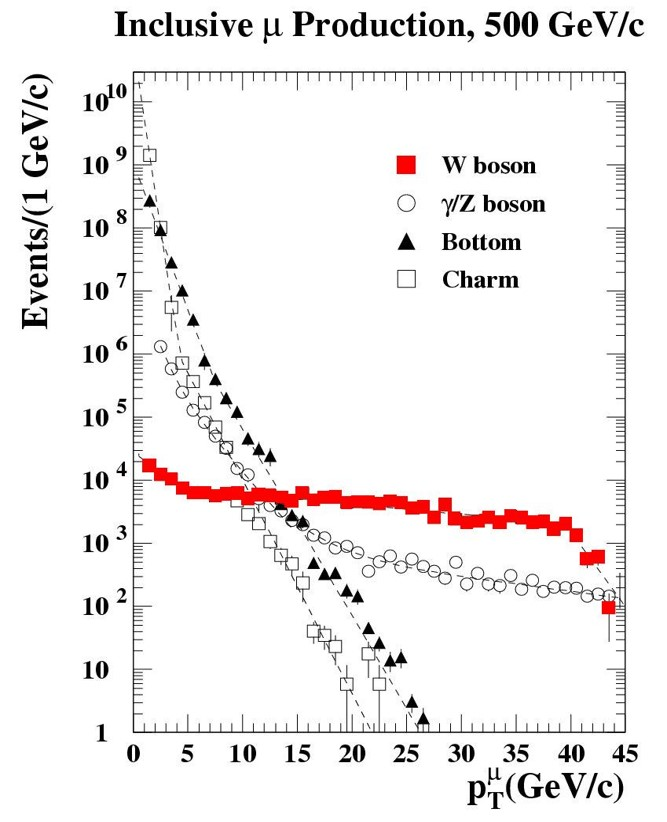
\includegraphics[width=0.5\linewidth]{../Chapter6/fig/muon_production_vs_pt.jpg}
		\caption{ Observing the simulated production of muon as a function of $p_T$, we
			can see that in the kinematic region of $W$ production that the dominant sources
			of muons come from other processes. The new PHENIX muon trigger threshold is
			sensitive at 10 $GeV/c$ and above. }
		\label{fig:muon_production_vs_pt}
	\end{center}
\end{figure}

We can divide up the total observed muon spectrum into contributions from three
sources:

\begin{itemize}
	\item Real Muon Background
		\begin{itemize}
			\item Z,$\gamma^*$
			\item $W\rightarrow$had
			\item $W\rightarrow$tau
		  \item onium
			\item open charm
			\item direct photon
		\end{itemize}
	\item Fake Muons (Hadronic Background)
		\begin{itemize}	
			\item Hadrons which are reconstructed as high $p_T$ muons due to detector
			resolution.
		\end{itemize}
	\item Signal Muons
		\begin{itemize}	
			\item Real $W\rightarrow\mu$ events.
		\end{itemize}
\end{itemize}

Previous analyses have attempted to separate the muon spectrum into $p_T$ bins,
to estimate the composition, however, because the $W\rightarrow\mu$ signal is so
small in the forward kinematic regime, these methods are not sufficient, as
there is no 'visible' cutoff in the spectrum. However, by using simulations.
However, we may use other methods to split up our spectrum, with the ultimate
goal of calculating $A_L$, and correcting for background dilution using the
signal to background ratio. We must use another method to effectively describe
the difference between an event which comes from a signal, vs background event.

\subsection{Naive Bayes Classification}
There are many techniques available for classifying a collection of variables
(a feature set) into categories. Naive Bayes classification is an excellent
candidate for classification, in cases where we have two classifications with
distributions of featuresets which are uncorrelated. Naive Bayes even works when
feature sets are slightly correlated. It is a robust, fast, scalable machine
learning technique. Traditionally used for classification of text documents,
Naive Bayes is also able to handle numeric features whose distributions are
known~\cite{Collins2013}.

In our analysis, we begin with a Naive Bayes classifer which is trained to
classify two signal muons, vs background muons. We combine both Real Muon
Background muons and Fake Muons (Hadronic Background Muons) in the label of
"Background Muons" at this stage, though, later, we will separate out the muons
further.

The descriniating variables described in~\ref{ch:data_collection} were
chosen from the multitude of possible physical event parameters, because they
were all maximally uncorrelated. Concretely, these correlations are presented in

\begin{figure}[H]
	\centering
	\begin{subfigure}{0.5\textwidth}
		\centering
		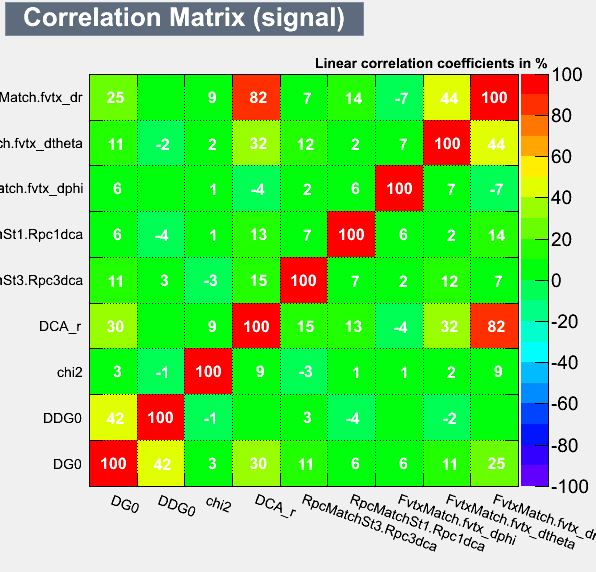
\includegraphics[width=0.95\linewidth]{../Chapter6/fig/CorrelationMatrix_Signal.png}
		\caption{Correlations between kinematic variables, produced from simulated
			data.}
		\label{fig:corr_mat_sig}
	\end{subfigure}%
	\begin{subfigure}{0.5\textwidth}
		\centering
		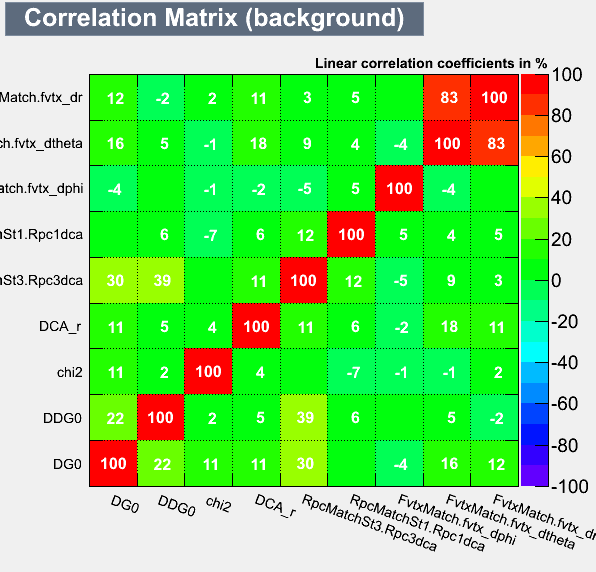
\includegraphics[width=0.95\linewidth]{../Chapter6/fig/CorrelationMatrix_Background.png}
		\caption{Correlations betwen kinematic variables, produced from the data,
			which is composed mostly of hadronic background}
		\label{fig:corr_mat_bkg}
	\end{subfigure}
	\caption{ Low correlations between the signal variable distributions (from
		simulation), and the background variable distributions make this data set a
		good candidate for classfication using Naive Bayes}
	\label{fig:kinematic_var_correlations}
\end{figure}

Briefly, a Naive Bayes classifier may be constructed from the core of the
familiar Bayes Theorem from probability and statistics.

In our case, we understand Naive Bayes as a conditional probability. Concretely,
we consider a vector of features (i.e. our discriminating kinematic variables):
\begin{equation}
	\label{eq:feature_vector}
\mathbf{x} = (x_1, \dots, x_n)
\end{equation}

and assume independence between each feature $x_n$. We then define the
probability of a given classification, $C_k$ given a set of features $x_n$:

\begin{equation}
	\label{eq:cond_probabilty}
p(C_k \vert x_1, \dots, x_n)
\end{equation}

This conditional probability is defined in terms of Bayes Theorem:

\begin{equation}
	\label{eq:bayes_theorm}
p(C_k \vert \mathbf{x}) = \frac{p(C_k) \ p(\mathbf{x} \vert C_k)}{p(\mathbf{x})}
\end{equation}

The terms here are defined as:
\begin{itemize}
	\item $p(C_k)\rightarrow$ prior probability
	\item $p(\mathbf{x} \vert C_k)\rightarrow$ likelihood
	\item $p(\mathbf{x})\rightarrow$ evidence
\end{itemize}

In principal, the final step in a classifier is to assign a class. This is done
by computing the probability of a feature-set belonging to one class, or to
another class, using Bayes Theroem. The class with the larger proability is than
taken as the defacto classification of that particular feature set. However, we
may instead observe these probabilities directly, and label data with this
probability. This is what we ultimately call our "$W_{ness}$" parameter. This
will be discussed in section~\ref{ssec:likelihood}.

\subsection{Composition of Probability Distribution Functions}
After we have engineered appropriate features to use in the analysis, we can
proceed with composing probability density functions so we can proceed with the
calculation of likelihoods, which will label our data set, allowing us to reduce
our data set further from the basic cuts, without removing any signal events.


\subsection{Labeling Data With Likliehood Ratio: $W_{ness}$}
\label{ssec:likelihood}
\section{Extended Unbinned Maximum Likelihood Fits}
\subsection{Modeling The Hadronic Background}
\subsection{Modeling the Muon Background}
\subsection{Modeling the W-Signal}
\subsection{Overview}
\subsection{Fit Performance}
\subsection{S/BG and Muon Backgrounds}
\label{ssec:sbr}
\subsection{$W_{ness}$ Dependence of S/BG}
\section{Calculation of $A_{L}$ for $W\rightarrow\mu$}
\subsection{Overview}
\subsection{Asymmetry Calculation}
\subsection{Discussion of Work Done By Analysis Team}
\section{Data Validation}
Mention Daniel's GPR, Ralf's PEPSI, Abraham's FVTX work, and Francesca's cross-checks.
\subsection{Simulations and The Signal to Background Ratio}
\subsection{Gaussian Process Regression}
\subsection{Four Way Cross Validation}
\subsection{Asymmetry Consistency Check}
\subsection{Beam Polarization}
\subsection{Beam Luminosity}
\subsection{Code Cross Validation}

\chapter{The Vernier Analysis}
\section{Overview}
\section{Analysis Note Here}
\section{W Cross Section}

\chapter{Discussion and Conclusion}


\nocite{*}
\bibliographystyle{plain}
\bibliography{mendeley.bib}
\appendix

\section{First Thingie}

\section{Second Thingie}


\end{document}
